\documentclass[a4paper]{article}

\def\npart {II}
\def\nterm {Michaelmas}
\def\nyear {2016}
\def\nlecturer {A.\ Ashton}
\def\ncourse {Integrable Systems}

\usepackage{myheader}

\begin{document}
\maketitle
{\small
\noindent\emph{Part IB Methods, and Complex Methods or Complex Analysis are essential; Part II Classical Dynamics is desirable.}

\vspace{10pt}
\noindent Integrability of ordinary differential equations: Hamiltonian systems and the Arnol'd--Liouville Theorem (sketch of proof). Examples.\hspace*{\fill}[3]

\vspace{5pt}
\noindent Integrability of partial differential equations: The rich mathematical structure and the universality of the integrable nonlinear partial differential equations (Korteweg-de Vries, sine--Gordon). Backlund transformations and soliton solutions.\hspace*{\fill}[2]

\vspace{5pt}
\noindent The inverse scattering method: Lax pairs. The inverse scattering method for the KdV equation, and other integrable PDEs. Multi soliton solutions. Zero curvature representation. \hspace*{\fill}[6]

\vspace{5pt}
\noindent Hamiltonian formulation of soliton equations.\hspace*{\fill}[2]

\vspace{5pt}
\noindent Painleve equations and Lie symmetries: Symmetries of differential equations, the ODE reductions of certain integrable nonlinear PDEs, Painleve equations.\hspace*{\fill}[3]%
}

\tableofcontents
\setcounter{section}{-1}
\section{Introduction}
What is an integrable system? Unfortunately, an integrable system is a something mathematicians have not yet managed to define properly. Intuitively, an integrable system is a differential equation we can ``integrate up'' directly. While in theory, integrable systems should be very rare, it happens that in nature, a lot of systems happen to be integrable. By exploiting the fact that they are integrable, we can solve them much more easily.

\section{Integrability of ODE's}
\subsection{Vector fields and flow maps}
In the first section, we are going to look at the integrability of ODE's. Here we are going to consider a general $m$-dimensional first order non-linear ODE's. As always, restricting to only first-order ODE's is not an actual restriction, since any higher-order ODE can be written as a system of first-order ODE's. At the end, we will be concerned with a special kind of ODE given by a \emph{Hamiltonian system}. However, in this section, we first give a quick overview of the general theory of ODEs.

An $m$-dimensional ODE is specified by a \term{vector field} $\mathbf{V}: \R^m \to \R^m$ and an \term{initial condition} $\mathbf{x}_0 \in \R^m$. The objective is to find some $\mathbf{x}(t) \in \R^m$, which is a function of $t \in (a, b)$ for some interval $(a, b)$ containing $0$, satisfying
\[
  \dot{\mathbf{x}} = \mathbf{V}(\mathbf{x}),\quad \mathbf{x}(0) = \mathbf{x}_0.
\]
In this course, we will assume the vector field $\mathbf{V}$ is sufficiently ``nice'', so that the following result holds:
\begin{fact}
  For a ``nice'' vector field $\mathbf{V}$ and any initial condition $\mathbf{x}_0$, there is always a unique solution to $\dot{\mathbf{x}} = \mathbf{V}(\mathbf{x})$, $\mathbf{x}(0) = \mathbf{x}_0$. Moreover, this solution depends smoothly (i.e.\ infinitely differentiably) on $t$ and $\mathbf{x}_0$.
\end{fact}

It is convenient to write the solution as
\[
  \mathbf{x}(t) = g^t \mathbf{x}_0,
\]
where $g^t: \R^m \to \R^m$ is called the \emph{flow map}. Since $\mathbf{V}$ is nice, we know this is a smooth map. This flow map has some nice properties:
\begin{prop}\leavevmode
  \begin{enumerate}
    \item $g^0 = \id$
    \item $g^{t + s} = g^t g^s$
    \item $(g^{t})^{-1} = g^{-t}$
  \end{enumerate}
\end{prop}
If one knows group theory, then this says that $g$ is a group homomorphism from $\R$ to the group of diffeomorphisms of $\R^m$, i.e.\ the group of smooth invertible maps $\R^m \to \R^m$.

\begin{proof}
  The equality $g^0 = \id$ is by definition of $g$, and the last equality follows from the first two since $t + (-t) = 0$. To see the second, we need to show that
  \[
    g^{t + s}\mathbf{x}_0 = g^t (g^s \mathbf{x}_0)
  \]
  for any $\mathbf{x}_0$. To do so, we see that both of them, as a function of $t$, are solutions to
  \[
    \dot{\mathbf{x}} = \mathbf{V}(\mathbf{x}),\quad \mathbf{x}(0) = g^s \mathbf{x}_0.
  \]
  So the result follows since solutions are unique.
\end{proof}

We say that $\mathbf{V}$ is the \term{infinitesimal generator} of the flow $g^t$. This is because we can Taylor expand.
\[
  \mathbf{x}(\varepsilon) = g^\varepsilon \mathbf{x}_0 = \mathbf{x}(0) + \varepsilon \dot{\mathbf{x}}(0) + o(\varepsilon) = \mathbf{x}_0 + \varepsilon \mathbf{V}(\mathbf{x}_0) + o(\varepsilon).
\]
Given vector fields $\mathbf{V}_1, \mathbf{V}_2$, one natural question to ask is whether their flows commute, i.e.\ if they generate $g_1^t$ and $g_2^s$, then must we have
\[
  g_1^t g_2^s \mathbf{x}_0 = g_2^s g_1^t \mathbf{x}_0
\]
for all $\mathbf{x}_0$? In general, this need not be true, so we might be interested to find out if this happens to be true for particular $\mathbf{V}_1, \mathbf{V}_2$. However, often, it is difficult to check this directly, because differential equations are generally hard to solve, and we will probably have a huge trouble trying to find explicit expressions for $g_1$ and $g_2$.

Thus, we would want to be able to consider this problem at an infinitesimal level, i.e.\ just by looking at $\mathbf{V}_1, \mathbf{V}_2$ themselves. It turns out the answer is given by the commutator:
\begin{defi}[Commutator]\index{commutator}
  For two vector fields $\mathbf{V}_1, \mathbf{V}_2: \R^m \to \R^m$, we define a third vector field called the \emph{commutator} by
  \[
    [\mathbf{V}_1, \mathbf{V}_2] = \left(\mathbf{V}_1 \cdot \frac{\partial}{\partial \mathbf{x}}\right) \mathbf{V}_2 - \left(\mathbf{V}_2 \cdot \frac{\partial}{\partial \mathbf{x}}\right) \mathbf{V}_1,
  \]
  where we write
  \[
    \frac{\partial}{\partial \mathbf{x}} = \left(\frac{\partial}{\partial x_1}, \cdots, \frac{\partial}{\partial x_n}\right)^T.
  \]
  More explicitly, the $i$th component is given by
  \[
    [\mathbf{V}_1, \mathbf{V}_2]_i = \sum_{j = 1}^m (\mathbf{V}_1)_j \frac{\partial}{\partial x_j} (\mathbf{V}_2)_i - (\mathbf{V}_2)_j \frac{\partial}{\partial x_j} (\mathbf{V}_1)_i
  \]
\end{defi}

The result we have is
\begin{prop}
  Let $\mathbf{V}_1, \mathbf{V}_2$ be vector fields with flows $g_1^t$ and $g_2^s$. Then we have
  \[
    [\mathbf{V}_1, \mathbf{V}_2] = 0 \quad\Longleftrightarrow\quad g_1^t g_2^s = g_2^s g_1^t.
  \]
\end{prop}

\begin{proof}
  See example sheet 1.
\end{proof}

\subsection{Hamiltonian dynamics}
From now on, we are going to restrict to a very special kind of ODE, known as a \emph{Hamiltonian system}. To write down a general ODE, the background setting is just the space $\R^n$. We then pick a vector field, and then we get an ODE. To write down a Hamiltonian system, we need more things in the background, but conversely we need to supply less information to get the system. These Hamiltonian system are very useful in classical dynamics, and our results here have applications in classical dynamics, but we will not go into the physical applications here.

The background settings of a Hamiltonian is a \term{phase space} $M = \R^{2n}$. Points on $M$ are described by coordinates
\[
  (\mathbf{q}, \mathbf{p}) = (q_1, \cdots, q_n, p_1, \cdots, p_n).
\]
We tend to think of the $q_i$ are ``generalized positions'' of particles, and the $p_n$ as the ``generalized momentum'' coordinates. We will often write
\[
  \mathbf{x} = (\mathbf{q}, \mathbf{p})^T.
\]
It is very important to note that here we have ``paired up'' each $q_i$ with the corresponding $p_i$. In normal $\R^n$, all the coordinates are equal, but this is no longer the case here. To encode this information, we define the $2n \times 2n$ anti-symmetric matrix
\[
  J =
  \begin{pmatrix}
    0 & I_n\\
    -I_n & 0
  \end{pmatrix}.
\]
We call this the \term{symplectic form}, and this is the extra structure we have for a phase space. We will later see that all the things we care about can be written in terms of $J$, but for practical purposes, we will often express them in terms of $\mathbf{p}$ and $\mathbf{q}$ instead.

The first example is the \emph{Poisson bracket}:

\begin{defi}[Poisson bracket]\index{Poisson bracket}
  For any two functions $f, g: M \to \R$, we define the \emph{Poisson bracket} by
  \[
    \{f, g\} = \frac{\partial f}{\partial \mathbf{x}} J \frac{\partial g}{\partial \mathbf{x}} = \frac{\partial f}{\partial \mathbf{q}} \cdot \frac{\partial g}{\partial \mathbf{p}} - \frac{\partial f}{\partial \mathbf{p}} \cdot \frac{\partial g}{\partial \mathbf{q}}.
  \]
\end{defi}

This has some obvious and not-so-obvious properties:
\begin{prop}\leavevmode
  \begin{enumerate}
    \item This is linear in each argument.
    \item This is antisymmetric, i.e.\ $\{f, g\} = - \{g, f\}$.
    \item This satisfies the Leibniz property:
      \[
        \{f, gh\} = \{f, g\}h + \{f, h\} g.
      \]
    \item This satisfies the Jacobi identity:
      \[
        \{f, \{g, h\}\} + \{g, \{h, f\}\} + \{h, \{f, g\}\} = 0.
      \]
    \item We have
      \[
        \{q_i, q_j\} = \{p_i, p_j\} = 0,\quad \{q_i, p_j\} = \delta_{ij}.
      \]
  \end{enumerate}
\end{prop}

\begin{proof}
  Just write out the definitions. In particular, you will be made to write out the 24 terms of the Jacobi identity in the first example sheet.
\end{proof}

We will be interested in problems on $M$ of the following form:
\begin{defi}[Hamilton's equation]\index{Hamilton's equation}
  \emph{Hamilton's equation} is an equation of the form
  \[
    \dot{\mathbf{q}} = \frac{\partial H}{\partial \mathbf{p}},\quad \dot{\mathbf{p}} = -\frac{\partial H}{\partial \mathbf{q}}\tag{$*$}
  \]
  for some function $H: M \to \R$ called the \term{Hamiltonian}.
\end{defi}
Just as we think of $\mathbf{q}$ and $\mathbf{p}$ as generalized position and momentum, we tend to think of $H$ as generalized energy.

Note that given the phase space $M$, all we need to specify a Hamiltonian system is just a Hamiltonian function $H: M \to \R$, which is much less information that that needed to specify a vector field.

In terms of $J$, we can write Hamilton's equation as
\[
  \dot{\mathbf{x}} = J \frac{\partial H}{\partial \mathbf{x}}.
\]
We can imagine Hamilton's equation as specifying the trajectory of a particle. In this case, we might want to ask how, say, the speed of the particle changes as it evolves. In general, suppose we have a smooth function $f: M \to \R$. We want to find the value of $\frac{\d f}{\d t}$. We simply have to apply the chain rule to obtain
\[
  \frac{\d f}{\d t} = \frac{\d}{\d t} f(\mathbf{x}(t)) = \frac{\partial f}{\partial \mathbf{x}} \cdot \dot{\mathbf{x}} = \frac{\partial f}{\partial \mathbf{x}} J \frac{\partial H}{\partial \mathbf{x}} = \{f, H\}.
\]
We record this result:
\begin{prop}
  Let $f: M \to \R$ be a smooth function. If $\mathbf{x}(t)$ evolves according to Hamilton's equation, then
  \[
    \frac{\d f}{\d t} = \{f, H\}.
  \]
\end{prop}
In particular, a function $f$ is constant if and only if $\{f, H\} = 0$. This is very convenient. Without a result like this, if we want to see if $f$ is a conserved quantity of the particle (i.e.\ $\frac{\d f}{\d t} = 0$), we might have to integrate the equations of motion, and then try to find explicitly what is conserved, or perhaps mess around with the equations of motion to somehow find that $\frac{\d f}{\d t}$ vanishes. However, we now have a very systematic way of figuring out if $f$ is a conserved quantity --- we just compute $\{f, H\}$.

In particular, we automatically find that the Hamiltonian is conserved:
\[
  \frac{\d H}{\d t} = \{H, H\} = 0.
\]
\begin{eg}
  Consider a particle (of unit mass) with position $\mathbf{q} = (q_1, q_2, q_3)$ (in Cartesian coordinates) moving under the influence of a potential $U(\mathbf{q})$. By Newton's second law, we have
  \[
    \ddot{\mathbf{q}} = -\frac{\partial U}{\partial \mathbf{q}}.
  \]
  This is actually a Hamiltonian system. We define the momentum variables by
  \[
    p_i = \dot{q}_i,
  \]
  then we have
  \[
    \dot{\mathbf{x}} =
    \begin{pmatrix}
      \dot{\mathbf{q}}\\
      \dot{\mathbf{p}}
    \end{pmatrix}
    =
    \begin{pmatrix}
      \mathbf{p}\\
      -\frac{\partial U}{\partial \mathbf{q}}
    \end{pmatrix}
    = J \frac{\partial H}{\partial \mathbf{x}},
  \]
  with
  \[
    H = \frac{1}{2} \abs{\mathbf{p}}^2 + U(\mathbf{q}).
  \]
  This is just the usual energy! Indeed, we can compute
  \[
    \frac{\partial H}{\partial \mathbf{p}} = \mathbf{p},\quad \frac{\partial H}{\partial \mathbf{q}} = \frac{\partial U}{\partial \mathbf{q}}.
  \]
\end{eg}

\begin{defi}[Hamiltonian vector field]\index{Hamiltonian vector field}
  Given a Hamiltonian function $H$, the \emph{Hamiltonian vector field} is given by
  \[
    \mathbf{V}_H = J \frac{\partial H}{\partial \mathbf{x}}.
  \]
\end{defi}

We then see that by definition, the Hamiltonian vector field generates the Hamiltonian flow. More generally, for any $f: M \to \R$, we call
\[
  \mathbf{V}_f = J \frac{\partial f}{\partial \mathbf{x}}.
\]
This is the Hamiltonian vector field with respect to $f$.

We know have two bracket-like things we can form. Given two $f, g$, we can take the Poisson bracket to get $\{f, g\}$, and consider its Hamiltonian vector field $\mathbf{V}_{\{f, g\}}$. On the other hand, we can first get $\mathbf{V}_f$ and $\mathbf{V}_g$, and then take the commutator of the vector fields. It turns out these are not equal, but differ by a sign.
\begin{prop}
  We have
  \[
    [\mathbf{V}_f, \mathbf{V}_g] = - \mathbf{\mathbf{V}}_{\{f, g\}}.
  \]
\end{prop}

\begin{proof}
  See first example sheet.
\end{proof}

\begin{defi}[First integral]\index{first integral}
  Given a phase space $M$ with a Hamiltonian $H$, we call $f: M \to \R$ a \emph{first integral} of the Hamiltonian system if
  \[
    \{f, H\} = 0.
  \]
\end{defi}
The reason for the term ``first integral'' is historical --- when we solve a differential equation, we integrate the equation. Every time we integrate it, we obtain a new constant. And the first constant we obtain when we integrate is known as the first integral. However, for our purposes, we can just as well think of it as a constant of motion.

\begin{eg}
  Consider the two-body problem --- the Sun is fixed at the origin, and a planet has Cartesian coordinates $\mathbf{q} = (q_1, q_2, q_3)$. The equation of motion will be
  \[
    \ddot{\mathbf{q}} = - \frac{\mathbf{q}}{|\mathbf{q}|^3}.
  \]
  This is equivalent to the Hamiltonian system $\mathbf{p} = \dot{\mathbf{q}}$, with
  \[
    H = \frac{1}{2} |\mathbf{p}|^2 - \frac{1}{|\mathbf{q}|}.
  \]
  We have an angular momentum given by
  \[
    \mathbf{L} = \mathbf{q} \wedge \mathbf{p}.
  \]
  Working with coordinates, we have
  \[
    L_i = \varepsilon_{ijk} q_j p_k.
  \]
  We then have (with implicit summation)
  \begin{align*}
    \{L_i, H\} &= \frac{\partial L_i}{\partial q_\ell}\frac{\partial H}{\partial p_\ell} - \frac{\partial L_i}{\partial p_\ell} \frac{\partial H}{\partial q_\ell}\\
    &= \varepsilon_{ijk} \left(p_k \delta_{\ell j}p_\ell + \frac{q_j q_k}{|\mathbf{q}|^3}\right)\\
    &= \varepsilon_{ijk} \left(p_k p_j + \frac{q_j q_k}{|\mathbf{q}|^3}\right)\\
    &= 0,
  \end{align*}
  where we know the thing vanishes because we contracted a symmetric tensor with an antisymmetric one. So this is a first integral.

  Less interestingly, we know $H$ is also a first integral. In general, some Hamiltonians have many many first integrals.
\end{eg}

Our objective of the remainder of the chapter is to show that if our Hamiltonian system has enough first integrals, then we can find a change of coordinates so that the equations of motion are ``trivial''. However, we need to impose some constraints on the integrals for this to be true. We will need to know about the following words:
\begin{defi}[Involution]\index{involution}
  We say that two first integrals $F, G$ are in \emph{involution} if $\{F, G\} = 0$ (so $F$ and $G$ ``\emph{Poisson commute}'').
\end{defi}

\begin{defi}[Independent first integrals]\index{independent first integrals}
  A collection of functions $f_i: M \to \R$ are independent if at each $\mathbf{x} \in M$, the vectors $\frac{\partial f_i}{\partial \mathbf{x}}$ for $i = 1, \cdots, n$ are independent.
\end{defi}

In general we will say a system is ``integrable'' if we can find a change of coordaintes so that the equations of motion become ``trivial'' and we can just integrate it up. This is a bit vague, so we will define integrability in terms of the existence of first integrals, and then we will later see that if these conditions are satisfied, then we can indeed integrate it up.:
\begin{defi}[Integrable system]\index{integrable system}
  A $2n$-dimensional Hamiltonian system $(M, H)$ is \emph{integrable} if there exists $n$ first integrals $\{f_i\}_{i = 1}^n$ that are independent and in involution (i.e.\ $\{f_i, f_j\} = 0$ for all $i, j$).
\end{defi}
The word independent is very important, or else people will cheat, e.g.\ take $H, 2H, e^H, H^2, \cdots$.

\begin{eg}
  Two-dimensional Hamiltonian systems are always integrable.
\end{eg}

\subsection{Canonical transformations}
We now come to the main result of the chapter. We will show that we can indeed integrate up integrable systems. We are going to show that there is a clever choice of coordinates such Hamilton's equations become ``trivial''. However, recall that the coordinates in a Hamiltonian system are not arbitrary. We have somehow ``paired up'' $q_i$ and $p_i$. So we want to only consider coordinate changes that somehow respect this pairing.

There are many ways we can define what it means to ``respect'' the pairing. We will pick a simple definition --- we require that it preserves the form of Hamilton's equation.

Suppose we had a general coordinate change $(\mathbf{q}, \mathbf{p}) \mapsto (\mathbf{Q}(\mathbf{q}, \mathbf{p}), \mathbf{P}(\mathbf{q}, \mathbf{p}))$.

\begin{defi}[Canonical transformation]\index{canonical transformation}
  A coordinate change $(\mathbf{q}, \mathbf{p}) \mapsto (\mathbf{Q}, \mathbf{P})$ is called \emph{canonical} if it leaves Hamilton's equations invariant, i.e.\ the equations in the original coordinates
  \[
    \dot{\mathbf{q}} = \frac{\partial H}{\partial \mathbf{q}},\quad \mathbf{p} = -\frac{\partial H}{\partial \mathbf{q}}.
  \]
  is equivalent to
  \[
    \dot{\mathbf{Q}} = \frac{\partial \tilde{H}}{\partial \mathbf{P}},\quad \dot{\mathbf{P}} = -\frac{\partial \tilde{H}}{\partial \mathbf{Q}},
  \]
  where $\tilde{H}(\mathbf{Q}, \mathbf{P}) = H(\mathbf{q}, \mathbf{p})$.
\end{defi}

If we write $\mathbf{x} = (\mathbf{q}, \mathbf{p})$ and $\mathbf{y} = (\mathbf{Q}, \mathbf{P})$, then this is equivalent to asking for
\[
  \dot{\mathbf{x}} = J \frac{\partial H}{\partial \mathbf{x}} \quad\Longleftrightarrow\quad \dot{\mathbf{y}} = J \frac{\partial \tilde{H}}{ \partial \mathbf{y}}.
\]
\begin{eg}
  If we just swap the $\mathbf{q}$ and $\mathbf{p}$ around, then the equations change by a sign. So this is not a canonical transformation.
\end{eg}

\begin{eg}
  The simplest possible case of a canonical transformation is a linear transformation. Consider a linear change of coordinates given by
  \[
    \mathbf{x} \mapsto \mathbf{y}(\mathbf{x}) = A\mathbf{x}.
  \]
  We claim that this is canonical iff $AJA^t = J$, i.e.\ that $A$ is \emph{symplectic}\index{symplectic transformation}.

  Indeed, by linearity, we have
  \[
    \dot{\mathbf{y}} = A\dot{\mathbf{x}} = AJ\frac{\partial H}{\partial \mathbf{x}}.
  \]
  Setting $\tilde{H}(\mathbf{y}) = H(\mathbf{x})$, we have
  \[
    \frac{\partial H}{\partial x_i} = \frac{\partial y_j}{\partial x_i} \frac{\partial \tilde{H}(\mathbf{y})}{\partial y_j} = A_{ji} \frac{\partial \tilde{H}(\mathbf{y})}{\partial y_j} = \left[A^T \frac{\partial \tilde{H}}{\partial \mathbf{y}}\right]_i.
  \]
  Putting this back in, we have
  \[
    \dot{\mathbf{y}} = AJA^T \frac{\partial\tilde{H}}{\partial \mathbf{y}}.
  \]
  So $\mathbf{y} \mapsto \mathbf{y}(\mathbf{x})$ is canonical iff $J = AJA^T$.
\end{eg}

What about more general cases? Recall from IB Analysis II that a differentiable map is ``locally linear''. Now Hamilton's equations are purely local equations, so we might expect the following:
\begin{prop}
  A map $\mathbf{x} \mapsto \mathbf{y}(\mathbf{x})$ is canonical iff $D\mathbf{y}$ is \emph{symplectic}\index{symplectic map}\index{symplectomorphism}, i.e.
  \[
    D\mathbf{y} J (D\mathbf{y})^T = J.
  \]
\end{prop}
Indeed, this follows from a simple application of the chain rule.

\subsubsection*{Generating functions}
We now discuss a useful way of producing canonical transformation, known as \term{generating functions}. In general, we can do generating functions in four different ways, but they are all very similar, so we will just do one that will be useful later on.

Suppose we have a function $S: \R^{2n} \to \R$. We suggestively write its arguments as $S(\mathbf{q}, \mathbf{P})$. We now set
\[
  \mathbf{p} = \frac{\partial S}{\partial \mathbf{q}},\quad \mathbf{Q} = \frac{\partial S}{\partial \mathbf{P}}.
\]
By this equation, we mean we write down the first equation, which allows us to solve for $\mathbf{P}$ in terms of $\mathbf{q}, \mathbf{p}$. Then the second equation tells us the value of $\mathbf{Q}$ in terms of $\mathbf{q}, \mathbf{P}$, hence in terms of $\mathbf{p}, \mathbf{q}$.

Usually, the way we use this is that we already have a candidate for what $\mathbf{P}$ should be. We then try to find a function $S(\mathbf{q}, \mathbf{P})$ such that the first equation holds. Then the second equation will tell us what the right choice of $\mathbf{Q}$ is.

Checking that this indeed gives rise to a canonical transformation is just a very careful application of the chain rule, which we shall not go into. Instead, we look at a few examples to see it in action.
\begin{eg}
  Consider the generating function
  \[
    S(\mathbf{q}, \mathbf{P}) = \mathbf{q} \cdot \mathbf{P}.
  \]
  Then we have
  \[
    \mathbf{p} = \frac{\partial S}{\partial \mathbf{q}} = \mathbf{P},\quad \mathbf{Q} = \frac{\partial S}{\partial \mathbf{P}} = \mathbf{q}.
  \]
  So this generates the identity transformation $(\mathbf{Q}, \mathbf{P}) = (\mathbf{q}, \mathbf{p})$.
\end{eg}

\begin{eg}
  In a 2-dimensional phase space, we consider the generating function
  \[
    S(q, P) = qP + q^2.
  \]
  Then we have
  \[
    p = \frac{\partial S}{\partial q} = P + 2q,\quad Q = \frac{\partial S}{\partial P} = q.
  \]
  So we have the transformation
  \[
    (Q, P) = (q, p - 2q).
  \]
  In matrix form, this is
  \[
    \begin{pmatrix}
      Q\\P
    \end{pmatrix} =
    \begin{pmatrix}
      1 & 0\\
      -2 & 1
    \end{pmatrix}
    \begin{pmatrix}
      q\\p
    \end{pmatrix}.
  \]
  To see that this is canonical, we compute
  \[
    \begin{pmatrix}
      1 & 0\\
      -2 & 1
    \end{pmatrix}
    J
    \begin{pmatrix}
      1 & 0\\
      -2 & 1
    \end{pmatrix}^T =
    \begin{pmatrix}
      1 & 0\\
      -2 & 1
    \end{pmatrix}
    \begin{pmatrix}
      0 & 1\\
      -1 & 0
    \end{pmatrix}
    \begin{pmatrix}
      1 & -2\\
      0 & 1
    \end{pmatrix} =
    \begin{pmatrix}
      0 & 1\\
      -1 & 0
    \end{pmatrix}
  \]
  So this is indeed a canonical transformation.
\end{eg}

\subsection{The Arnold-Liouville theorem}
We now get to the Arnold-Liouville theorem. This theorem says that if a Hamiltonian system is integrable, then we can find a canonical transformation $(\mathbf{q}, \mathbf{p}) \mapsto (\mathbf{Q}, \mathbf{P})$ such that $\tilde{H}$ depends only on $\mathbf{P}$. If this happened, then Hamilton's equations reduce to
\[
  \dot{\mathbf{Q}} = \frac{\partial \tilde{H}}{\partial \mathbf{P}},\quad \dot{\mathbf{P}} = -\frac{\partial \tilde{H}}{\partial \mathbf{Q}} = 0,
\]
which is pretty easy to solve. We find that $\mathbf{P}(t) = \mathbf{P}_0$ is a constant, and since the right hand side of the first equation depends only on $\mathbf{P}$, we find that $\dot{\mathbf{Q}}$ is also constant! So $\mathbf{Q} = \mathbf{Q}_0 + \Omega t$, where
\[
  \Omega = \frac{\partial \tilde{H}}{\partial \mathbf{P}} (\mathbf{P}_0).
\]
So the solution just falls out very easily.

Before we prove the Arnold-Liouville theorem in full generality, we first see how the canonical transformation looks like in a very particular case. Here we will just have to write down the canonical transformation and see that it works, but we will later find that the Arnold-Liouville theorem give us a general method to find the transformation.

\begin{eg}
  Consider the harmonic oscillator with Hamiltonian
  \[
    H(q, p) = \frac{1}{2}p^2 + \frac{1}{2}\omega^2 q^2.
  \]
  Since is a 2-dimensional system, so we only need a single first integral. Since $H$ is a first integral for trivial reasons, this is an integrable Hamiltonian system.

  We can actually draw the lines on which $H$ is constant --- they are just ellipses:
  \begin{center}
    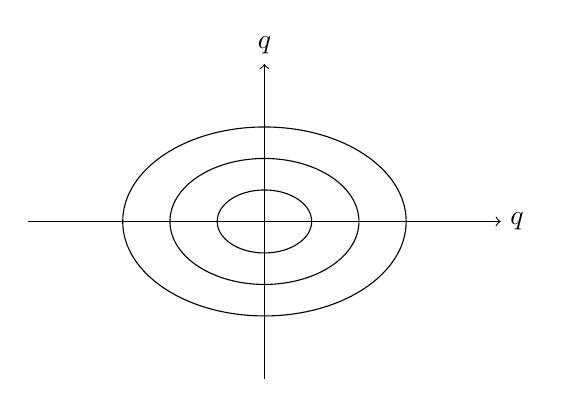
\begin{tikzpicture}
      \draw [->] (-3, 0) -- (3, 0) node [right] {$q$};
      \draw [->] (0, -2) -- (0, 2) node [above] {$q$};

      \foreach \x in {0.4, 0.8, 1.2} {
        \begin{scope}[scale=\x]
          \draw ellipse (1.5 and 1);
        \end{scope}
      }
    \end{tikzpicture}
  \end{center}
  We note that the ellipses are each homeomorphic to $S^1$. Now we introduce the coordinate transformation $(q, p) \mapsto (\phi, I)$, defined by
  \[
    q = \sqrt{\frac{2I}{\omega}} \sin \phi,\quad p = \sqrt{2I\omega} \cos \phi,
  \]
  For the purpose of this example, we can suppose we obtained this formula through divine inspiration. However, in the Arnold-Liouville theorem, we will provide a general way of coming up with these formulas.

  We can manually show that this transformation is canonical, but it is merely a computation and we will not waste time doing that. IN these new coordinates, the Hamiltonian looks like
  \[
    \tilde{H}(\phi, I) = H(q(\phi, I), p(\phi, I)) = \omega I.
  \]
  This is really nice. There is no $\phi$! Now Hamilton's equations become
  \[
    \dot\phi = \frac{\partial \tilde{H}}{ \partial I} = \omega,\quad \dot{I} = -\frac{\partial \tilde{H}}{\partial \phi} = 0.
  \]
  We can integrate up to obtain
  \[
    \phi(t) = \phi_0 + \omega t,\quad I(t) = I_0.
  \]
  For some unexplainable reason, we decide it is fun to consider the integral along paths of constant $H$:
  \begin{align*}
    \frac{1}{2\pi}\oint p \;\d q &= \frac{1}{2\pi} \int_0^{2\pi}p(\phi, I) \left(\frac{\partial q}{\partial \phi} \;\d \phi + \frac{\partial q}{\partial I} \;\d I\right)\\
    &= \frac{1}{2\pi} \int_0^{2\pi}p(\phi, I) \left(\frac{\partial q}{\partial \phi} \;\d \phi\right)\\
    &= \frac{1}{2\pi} \int_0^{2\pi} \sqrt{\frac{2I}{\omega}}\sqrt{2I\omega} \cos^2 \phi \;\d \phi\\
    &= I
  \end{align*}
  This is interesting. We could always have performed the integral $\frac{1}{2\pi} \oint p \;\d q$ along paths of constant $H$ without knowing anything about $I$ and $\phi$, and this would have magically gave us the new coordinate $I$.
\end{eg}

There are two things to take away from this.
\begin{enumerate}
  \item The motion takes place in $S^1$
  \item We got $I$ by performing $\frac{1}{2\pi}\oint p \;\d q$.
\end{enumerate}
These two ideas are essentially what we are going to prove for general Hamiltonian system.

\begin{thm}[Arnold-Liouville theorem]\index{Arnold-Liouville theorem}
  We let $(M, H)$ be an integrable $2n$-dimensional Hamiltonian system with independent, involutive first integrals $f_1, \cdots, f_n$, where $f_1 = H$. For any fixed $\mathbf{c} \in \R^n$, we set
  \[
    M_\mathbf{c} = \{(\mathbf{q}, \mathbf{p}) \in M: f_i(\mathbf{q}, \mathbf{p}) = c_i, i =1 , \cdots, n\}.
  \]
  Then
  \begin{enumerate}
    \item $M_\mathbf{c}$ is a smooth $n$-dimensional surface in $M$. If $M_\mathbf{c}$ is compact and connected, then it is diffeomorphic to
      \[
        T^n = S^1 \times \cdots \times S^1.
      \]
    \item If $M_\mathbf{c}$ is compact and connected, then locally, there exists canonical coordinate transformations $(\mathbf{q}, \mathbf{p}) \mapsto (\boldsymbol\phi, \mathbf{I})$ called the \term{action-angle coordinates} such that the angles $\{\phi_k\}_{k = 1}^n$ are coordinates on $M_\mathbf{c}$; the actions $\{I_k\}_{k = 1}^n$ are first integrals, and $H(\mathbf{q}, \mathbf{p})$ does not depend on $\boldsymbol\phi$. In particular, Hamilton's equations
      \[
        \dot{\mathbf{I}} = 0,\quad \dot{\boldsymbol\phi} = \frac{\partial \tilde{H}}{\partial \mathbf{I}} = \text{constant}.
      \]
  \end{enumerate}
\end{thm}

Some parts of the proof will refer to certain results from rather pure courses, which the applied people may be willing to just take on faith.
\begin{proof}[Proof sketch]
  The first part is pure differential geometry. To show that $M_\mathbf{c}$ is smooth and $n$-dimensional, we apply the preimage theorem you may or may not have learnt from IID Differential Geometry (which is in turn an easy consequence of the inverse function theorem from IB Analysis II). The key that makes this work is that the constraints are independent, which is the condition that allows the preimage theorem to apply.

  We next show that $M_\mathbf{c}$ is diffeomorphic to the torus if it is compact and connected. Consider the Hamiltonian vector fields defined by
  \[
    \mathbf{V}_{f_i} = J \frac{\partial f_i}{\partial \mathbf{x}}.
  \]
  We claim that these are \emph{tangent} to the surface $M_\mathbf{c}$. By differential geometry, it suffices to show that the derivative of the $\{f_j\}$ in the direction of $\mathbf{V}_{f_i}$ vanishes. We can compute
  \[
    \left(\mathbf{V}_{f_i} \cdot \frac{\partial}{\partial \mathbf{x}}\right)f_j = \frac{\partial f_j}{\partial \mathbf{x}} J \frac{\partial f_i}{\partial \mathbf{x}} = \{f_j, f_i\} = 0.
  \]
  Since this vanishes, we know that $\mathbf{V}_{f_i}$ is a tangent to the surface. Again by differential geometry, the flow maps $\{g_i\}$ must map $M_\mathbf{c}$ to itself. Also, we know that the flow maps commute. Indeed, this follows from the fact that
  \[
    [\mathbf{V}_{f_i}, \mathbf{V}_{f_j}] = -\mathbf{V}_{\{f_i, f_j\}} = -\mathbf{V}_{0} = 0.
  \]
  So we have a whole bunch of commuting flow maps from $M_\mathbf{c}$ to itself. We set
  \[
    g^\mathbf{t} = g_1^{t_1} g_2^{t_2} \cdots g_n^{t_n},
  \]
  where $\mathbf{t} \in \R^n$. Then because of commutativity, we have
  \[
    g^{\mathbf{t}_1 + \mathbf{t}_2} = g^{\mathbf{t}_1}g^{\mathbf{t}_2}.
  \]
  So this is gives a group action of $\R^n$ on the surface $M_\mathbf{c}$. We fix $\mathbf{x} \in M_\mathbf{c}$. We define
  \[
    \stab(\mathbf{x}) = \{\mathbf{t} \in \R^n: g^\mathbf{t}\mathbf{x} = \mathbf{x}\}.
  \]
  We introduce the map
  \[
    \phi: \frac{\R^n}{\stab(\mathbf{x})} \to M_\mathbf{c}
  \]
  given by $\phi(\mathbf{t}) = g^{\mathbf{t}}\mathbf{x}$. By the orbit-stabilizer theorem, this gives a bijection between $\R^n/\stab(\mathbf{x})$ and the orbit of $\mathbf{x}$. It can be shown that the orbit of $\mathbf{x}$ is exactly the connected component of $\mathbf{x}$. Now if $M_\mathbf{c}$ is connected, then this must be the whole of $\mathbf{x}$! By general differential geometry theory, we get that this map is indeed a diffeomorphism.

  We know that $\stab(\mathbf{x})$ is a subgroup of $\R^n$, and if the $g_i$ are non-trivial, it can be seen (at least intuitively) that this is discrete. Thus, it must be isomorphic to something of the form $\Z^k$ with $1 \leq k \leq n$.

  So we have
  \[
    M_\mathbf{c} \cong \R^n / \stab(\mathbf{x}) \cong \R^n/\Z^k \cong \R^k/\Z^k \times \R^{n - k} \cong T^k \times \R^{n - k}.
  \]
  Now if $M_\mathbf{c}$ is compact, we must have $n - k = 0$, i.e.\ $n = k$, so that we have no factors of $\R$. So $M_\mathbf{c} \cong T^n$.

  \separator

  With all the differential geometry out of the way, we can now construct the action-angle coordinates.

  For simplicity of presentation, we only do it in the case when $n = 2$. The proof for higher dimensions is entirely analogous, except that we need to use a higher-dimensional analogue of Green's theorem, which we do not currently have.

  We note that it is currently trivial to re-parameterize the phase space with coordinates $(\mathbf{Q}, \mathbf{P})$ such that $\mathbf{P}$ is constant within the Hamiltonian flow, and each coordinate of $\mathbf{Q}$ takes values in $S^1$. Indeed, we just put $\mathbf{P} = \mathbf{c}$ and use the diffeomorphism $T^n \cong M_\mathbf{c}$ to parameterize each $M_\mathbf{c}$ as a product of $n$ copies of $S^n$. However, this is not good enough, because such an arbitrary transformation will almost certainly not be canonical. So we shall try to find a more natural and in fact canonical way of parametrizing our phase space.

  We first work on the generalized momentum part. We want to replace $\mathbf{c}$ with something nicer. We will do something analogous to the simple harmonic oscillator we've got.

  So we fix a $\mathbf{c}$, and try to come up with some numbers $\mathbf{I}$ that labels this $M_\mathbf{c}$. Recall that our surface $M_\mathbf{c}$ looks like a torus:
  \begin{center}
    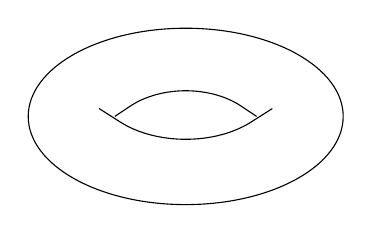
\begin{tikzpicture}
      \draw (0,0) ellipse (2 and 1.12);
      \path[rounded corners=24pt] (-.9,0)--(0,.6)--(.9,0) (-.9,0)--(0,-.56)--(.9,0);
      \draw[rounded corners=28pt] (-1.1,.1)--(0,-.6)--(1.1,.1);
      \draw[rounded corners=24pt] (-.9,0)--(0,.6)--(.9,0);
    \end{tikzpicture}
  \end{center}
  Up to continuous deformation of loops, we see that there are two non-trivial ``single'' loops in the torus, given by the red and blue loops:
  \begin{center}
    \begin{tikzpicture}
      \draw (0,0) ellipse (2 and 1.12);
      \draw [mred] (0,0) ellipse (1.5 and 0.6);

      \draw [mblue] (0, -0.71) ellipse (0.1 and 0.41);
      \draw [rounded corners=28pt] (-1.1,.1)--(0,-.6)--(1.1,.1);
      \draw [rounded corners=24pt] (-.9,0)--(0,.6)--(.9,0);
    \end{tikzpicture}
  \end{center}
  More generally, for an $n$ torus, we have $n$ such distinct loops $\Gamma_1, \cdots, \Gamma_n$. More concretely, after identifying $M_\mathbf{c}$ with $S^n$, these are the loops given by
  \[
    \{0\} \times \cdots \times \{0\} \times S^1 \times \{0\} \times \cdots \times \{0\} \subseteq S^1.
  \]
  We now attempt to define:
  \[
    I_j = \frac{1}{2\pi} \oint_{\Gamma_j} \mathbf{p}\cdot \d \mathbf{q},
  \]
  This is just like the formula we had for the simple harmonic oscillator.

  We want to make sure this is well-defined --- recall that $\Gamma_i$ actually represents a \emph{class} of loops identified under continuous deformation. What if we picked a different loop?
  \begin{center}
    \begin{tikzpicture}
      \draw (0,0) ellipse (2 and 1.12);
      \draw [mblue] (0.5, -1.09) arc (270:450:0.1 and 0.43);
      \draw [mblue, dashed] (0.5, -0.23) arc (90:270:0.1 and 0.43);
      \draw [mblue, dashed] (-0.5, -1.09) arc (270:450:0.1 and 0.43);
      \draw [mblue] (-0.5, -0.23) arc (90:270:0.1 and 0.43);

      \node [mblue, right] at (0.6, -0.66) {$\Gamma_2'$};
      \node [mblue, left] at (-0.6, -0.66) {$\Gamma_2$};
      \draw [rounded corners=28pt] (-1.1,.1)--(0,-.6)--(1.1,.1);
      \draw [rounded corners=24pt] (-.9,0)--(0,.6)--(.9,0);
    \end{tikzpicture}
  \end{center}
  On $M_\mathbf{c}$, we have the equation
  \[
    f_i(\mathbf{q}, \mathbf{p}) = \mathbf{c}_i.
  \]
  We will have to assume that we can invert this equation for $\mathbf{p}$ locally, i.e.\ we can write
  \[
    \mathbf{p} = \mathbf{p}(\mathbf{q}, \mathbf{c}).
  \]
  The condition for being able to do so is just
  \[
    \det\left(\frac{\partial f_i}{\partial p_j}\right) \not= 0,
  \]
  which is not hard.

  Then by definition, the following holds identically:
  \[
    f_i(\mathbf{q}, \mathbf{p}(\mathbf{q}, \mathbf{c})) = c_i.
  \]
  We an then differentiate this with respect to $q_k$ to obtain
  \[
    \frac{\partial f_i}{\partial q_k} + \frac{\partial f_i}{\partial p_\ell} \frac{\partial p_\ell}{\partial q_k} = 0
  \]
  on $M_\mathbf{c}$. Now recall that the $\{f_i\}$'s are in involution. So on $M_\mathbf{c}$, we have
  \begin{align*}
    0 &= \{f_i, f_j\} \\
    &= \frac{\partial f_i}{\partial q_k} \frac{\partial f_j}{\partial p_k} - \frac{\partial f_i}{\partial p_k} \frac{\partial f_j}{\partial q_k}\\
    &= \left(-\frac{\partial f_i}{\partial p_\ell} \frac{\partial p_\ell}{\partial q_k}\right)\frac{\partial f_j}{\partial p_k} - \frac{\partial f_i}{\partial p_k}\left(-\frac{\partial f_j}{\partial p_\ell} \frac{\partial p_\ell}{\partial q_k}\right)\\
    &= \left(-\frac{\partial f_i}{\partial p_k} \frac{\partial p_k}{\partial q_\ell}\right)\frac{\partial f_j}{\partial p_\ell} - \frac{\partial f_i}{\partial p_k}\left(-\frac{\partial f_j}{\partial p_\ell} \frac{\partial p_\ell}{\partial q_k}\right)\\
    &= \frac{\partial f_i}{\partial p_k} \left(\frac{\partial p_\ell}{\partial q_k} - \frac{\partial p_k}{\partial q_\ell}\right) \frac{\partial f_j}{\partial p_\ell}.
  \end{align*}
  Recall that the determinants of the matrices $\frac{\partial f_i}{\partial p_k}$ and $\frac{\partial f_j}{\partial p_\ell}$ are non-zero, i.e.\ the matrices are invertible. So for this to hold, the middle matrix must vanish! So we have
  \[
    \frac{\partial p_\ell}{\partial q_k} - \frac{\partial p_k}{\partial q_\ell} = 0.
  \]
  In our particular case of $n = 2$, since $\ell, k$ can only be $1, 2$, the only non-trivial thing this says is
  \[
    \frac{\partial p_1}{\partial q_2} - \frac{\partial p_2}{\partial q_1} = 0.
  \]
  Now suppose we have two ``simple'' loops $\Gamma_2$ and $\Gamma_2'$. Then they bound an area $A$:
  \begin{center}
    \begin{tikzpicture}
      \draw (0,0) ellipse (2 and 1.12);
      \draw [mblue] (0.5, -1.09) arc (270:450:0.1 and 0.43);
      \draw [mblue, dashed] (0.5, -0.23) arc (90:270:0.1 and 0.43);
      \draw [mblue, dashed] (-0.5, -1.09) arc (270:450:0.1 and 0.43);
      \draw [mblue] (-0.5, -0.23) arc (90:270:0.1 and 0.43);

      \node [mblue, right] at (0.6, -0.66) {$\Gamma_2'$};
      \node [mblue, left] at (-0.6, -0.66) {$\Gamma_2$};
      \draw [rounded corners=28pt] (-1.1,.1)--(0,-.6)--(1.1,.1);
      \draw [rounded corners=24pt] (-.9,0)--(0,.6)--(.9,0);

      \fill [morange, opacity=0.3] (0.5, -1.09) arc (270:450:0.1 and 0.43) to [out=190, in=-10] (-0.5, -0.23) arc (90:270:0.1 and 0.43) to [out=-7, in=187] (0.5, -1.09);

      \node [morange!50!black] at (0, -0.71) {$A$};
    \end{tikzpicture}
  \end{center}
  Then we have
  \begin{align*}
    \left(\oint_{\Gamma_2} - \oint_{\Gamma_2'}\right) \mathbf{p}\cdot \d \mathbf{q} &= \oint_{\partial A}\mathbf{p}\cdot \d \mathbf{q}\\
    &= \iint_A \left(\frac{\partial p_2}{\partial q_1} - \frac{\partial p_1}{\partial q_2}\right) \;\d q_1\;\d q_2\\
    &= 0
  \end{align*}
  by Green's theorem.

  So $I_j$ is well-defined, and
  \[
    \mathbf{I} = \mathbf{I}(\mathbf{c})
  \]
  is just a function of $c$. This will be our new ``momentum'' coordinates. To figure out what the angles $\boldsymbol\phi$ should be, we use generating functions. For now, we assume that we can invert $\mathbf{I}(\mathbf{c})$, so that we can write
  \[
    \mathbf{c} = \mathbf{c}(\mathbf{I}).
  \]
  We arbitrarily pick a point $\mathbf{x}_0$, and define the generating function
  \[
    S(\mathbf{q}, \mathbf{I}) = \int_{\mathbf{x}_0}^\mathbf{x} \mathbf{p}(\mathbf{q}', \mathbf{c}(\mathbf{I})) \cdot \d \mathbf{q}',
  \]
  where $\mathbf{x} = (\mathbf{q}, \mathbf{p}) = (\mathbf{q}, \mathbf{p}(\mathbf{q}, \mathbf{c}(\mathbf{I})))$. However, this is not \emph{a priori} well-defined, because we haven't said how we are going to integrate from $\mathbf{x}_0$ to $\mathbf{x}$. We are going to pick paths arbitrarily, but we want to make sure it is well-defined. Suppose we change from a path $\gamma_1$ to $\gamma_2$ by a little bit, and they enclose a surface $B$.
  \begin{center}
    \begin{tikzpicture}
      \node [circ] {};
      \node [left] {$\mathbf{x}_0$};
      \node at (2, 2) [circ] {};
      \node at (2, 2) [right] {$\mathbf{x}$};
      \node at (2, 1) {$\gamma_2$};
      \draw [->-=0.6] plot [smooth, tension=1] coordinates {(0, 0) (0.8, 1.7) (2, 2)};
      \node [above] at (0.8, 1.7) {$\gamma_1$};
      \draw [->-=0.6] plot [smooth, tension=1] coordinates {(0, 0) (1.2, -0.1) (2, 2)};
      \node at (1, 0.9) {$B$};
    \end{tikzpicture}
  \end{center}
  Then we have
  \[
    S(\mathbf{q}, \mathbf{I}) \mapsto S(\mathbf{q}, \mathbf{I}) + \oint_{\partial B} \mathbf{p} \cdot \d \mathbf{q}.
  \]
  Again, we are integrating $\mathbf{p} \cdot \d\mathbf{q}$ around a boundary, so there is no change.

  However, we don't live in flat space. We live in a torus, and we can have a crazy loop that does something like this:
  \begin{center}
    \begin{tikzpicture}
      \draw (-3, 1) to [out=5, in=175] (3, 1);
      \draw (-3, -1) to [out=5, in=175] (3, -1);

      \node (i) [circ] at (-1, 0) {};
      \node (f) [circ] at (1, 0.2) {};

      \draw [mblue, ->-=0.5] (i) to [out=10, in=150] (f);

      \draw [mred] (i) to [out=30, in=180] (0, 1.15);

      \draw [mred, dashed, ->-=0.7] (0, 1.15) arc(90:-90:0.1 and 1);

      \draw [mred] (0, -0.85) to [out=180, in=180] (f);
    \end{tikzpicture}
  \end{center}
  Then what we have effectively got is that we added a loop (say) $\Gamma_2$ to our path, and this contributes a factor of $2\pi I_2$. In general, these transformations give changes of the form
  \[
    S(\mathbf{q}, \mathbf{I}) \mapsto S(\mathbf{q}, \mathbf{I}) + 2\pi I_j.
  \]
  This is the only thing that can happen. So differentiating with respect to $I$, we know that
  \[
    \boldsymbol\phi = \frac{\partial S}{\partial \mathbf{I}}
  \]
  is well-defined modulo $2\pi$. These are the \emph{angles coordinates}. Note that just like angles, we can pick $\boldsymbol\phi$ consistently locally without this ambiguity, as long as we stay near some fixed point, but when we want to talk about the whole surface, this ambiguity necessarily arises. Now also note that
  \[
    \frac{\partial S}{\partial \mathbf{q}} = \mathbf{p}.
  \]
  Indeed, we can write
  \[
    S = \int_{\mathbf{x}_0}^\mathbf{x} \mathbf{F} \cdot \d \mathbf{x}',
  \]
  where
  \[
    \mathbf{F} = (\mathbf{p}, 0).
  \]
  So by the fundamental theorem of calculus, we have
  \[
    \frac{\partial S}{\partial \mathbf{x}} = \mathbf{F}.
  \]
  So we get that
  \[
    \frac{\partial S}{\partial \mathbf{q}} = \mathbf{p}.
  \]
  In summary, we have constructed on $M_\mathbf{c}$ the following: $\mathbf{I}= \mathbf{I}(\mathbf{c})$, $S(\mathbf{q}, I)$, and
  \[
    \boldsymbol\phi = \frac{\partial S}{\partial \mathbf{I}},\quad \mathbf{p} = \frac{\partial S}{\partial \mathbf{q}}.
  \]
  So $S$ is a generator for the canonical transformation, and $(\mathbf{q}, \mathbf{p}) \mapsto (\boldsymbol\phi, \mathbf{I})$ is a canonical transformation.

  Note that at any point $\mathbf{x}$, we know $\mathbf{c} = \mathbf{f}(\mathbf{x})$. So $I(\mathbf{c}) = I(\mathbf{f})$ depends on the first integrals only. So we have
  \[
    \dot{\mathbf{I}} = 0.
  \]
  So Hamilton's equations become
  \[
    \dot{\boldsymbol\phi} = \frac{\partial \tilde{H}}{\partial \mathbf{I}},\quad \dot{\mathbf{I}} = 0 = \frac{\partial \tilde{H}}{\partial \boldsymbol\phi}.
  \]
  So the new Hamiltonian depends only on $\mathbf{I}$. So we can integrate up and get
  \[
    \boldsymbol\phi(t) = \boldsymbol\phi_0 + \Omega t,\quad \mathbf{I}(t) = \mathbf{I}_0,
  \]
  where
  \[
    \Omega = \frac{\partial\tilde{H}}{\partial \mathbf{I}}(\mathbf{I}_0).\qedhere
  \]
\end{proof}
To summarize, to integrate up an integrable Hamiltonian system, we identify the different cycles $\Gamma_1, \cdots, \Gamma_n$ on $M_\mathbf{c}$. We then construct
\[
  I_j = \frac{1}{2\pi} \oint_{\Gamma_j} \mathbf{p}\cdot \d \mathbf{q},
\]
where $\mathbf{p} = \mathbf{p}(\mathbf{q}, \mathbf{c})$. We then invert this to say
\[
  \mathbf{c} = \mathbf{c}(\mathbf{I}).
\]
We then compute
\[
  \boldsymbol\phi = \frac{\partial S}{\partial \mathbf{I}},
\]
where
\[
  S = \int_{\mathbf{x}_0}^{\mathbf{x}} \mathbf{p}(\mathbf{q}', \mathbf{c}(\mathbf{I})) \cdot \d \mathbf{q}'.
\]
Now we do this again with the Harmonic oscillator.
\begin{eg}
  In the harmonic oscillator, we have
  \[
    H(q, p) = \frac{1}{2}p^2 + \frac{1}{2}\omega^2 q^2.
  \]
  We then have
  \[
    M_\mathbf{c} = \left\{(q, p): \frac{1}{2} p^2 + \frac{1}{2}\omega^2 q^2 = c\right\}.
  \]
  The first part of the Arnold-Liouville theorem says this is diffeomorphic to $T^1 = S^1$, which it is! The next step is to pick a loop, and there is an obvious one --- the circle itself. We write
  \[
    p = p(q, c) = \pm \sqrt{2c - \omega^2 q^2}
  \]
  on $M_\mathbf{c}$. Then we have
  \[
    I = \frac{1}{2\pi} \int p \cdot \d q = \frac{c}{\omega}.
  \]
  We can then write $c$ as a function of $I$ by
  \[
    c = c(I) = \omega I.
  \]
  Now construct
  \[
    S(q, I) = \int_{x_0}^{x} p(q', c(I))\;\d q'.
  \]
  We can pick $x_0$ to be the point corresponding to $\theta = 0$. Then this is equal to
  \[
    \int_0^q \sqrt{2\omega I - \omega^2 q'^2} \;\d q'.
  \]
  To find $\phi$, we need to differentiate this thing to get
  \[
    \phi = \frac{\partial S}{\partial I} = \omega\int_0^q \frac{\d q'}{\sqrt{2 \omega I - \omega^2 q'^2}} = \sin^{-1}\left(\sqrt{\frac{\omega}{2I}}q\right)
  \]
  As expected, this is only well-defined up to a factor of $2\pi$! Using the fact that $c = H$, we have
  \[
    q = \sqrt{\frac{2\pi}{\omega}} \sin \phi,\quad p = \sqrt{2I\omega} \cos \phi.
  \]
  These are exactly the coordinates we obtained through divine inspiration last time.
\end{eg}
\section{Partial Differential Equations}
For the remainder of the course, we are going to look at PDE's. We can view these as infinite-dimensional analogues of ODE's. So what do we expect for integrable PDE's? Recall that If an $2n$-dimensional ODE is integrable, then we $n$ first integrals. Since PDE's are infinite-dimensional, and half of infinity is still infinity, we would expect to have infinitely many first integrals. Similar to the case of integrable ODE's, we would also expect that there will be some magic transformation that allows us to write down the solution with ease, even if the initial problem looks very complicated.

These are all true, but our journey will be less straightforward. To begin with, we will not define what integrability means, because it is a rather complicated issue. We will go through one method of ``integrating up'' a PDE in detail, known as the inverse scattering transform, and we will apply it to a particular equation. Unfortunately, the way we apply the inverse scattering transform to a PDE is not obvious, and here we will have to do it through ``divine inspiration''.

Before we get to the inverse scattering transform, we first look at a few examples of PDEs.

\subsection{KdV equation}
The \term{KdV equation} is given by
\[
  u_t + u_{xxx} - 6 u u_x = 0.
\]
Before we study the KdV equation, we will look at some variations of this where we drop some terms, and then see how they compare.

\begin{eg}
  Consider the linear PDE
  \[
    u_t + u_{xxx} = 0,
  \]
  where $u = u(x, t)$ is a function on two variables. This admits solutions of the form
  \[
    e^{ikx - i\omega t},
  \]
  known as \term{plane wave modes}. For this to be a solution, $\omega$ must obey the \term{dispersion relation}
  \[
    \omega = \omega(k) = -k^3.
  \]
  For \emph{any} $k$, as long as we pick $\omega$ this way, we obtain a solution. By writing the solution as
  \[
    u(x, t) = \exp\left(ik\left(x - \frac{\omega(k)}{k}t\right)\right),
  \]
  we see that plane wave modes travel at speed
  \[
    \frac{\omega}{k} = -k^2.
  \]
  It is very important that the speed depends on $k$. Different plane wave modes travel at different speeds. This is going to give rise to what we call \term{dispersion}.

  A general solution is a superposition of plane wave modes
  \[
    \sum_k a(k) e^{ikx - i \omega(k) t},
  \]
  or even an uncountable superposition
  \[
    \int_k A(k) e^{ikx - i\omega(k)t}\;\d k.
  \]
  It is a theorem that for linear PDE's on convex domains, all solutions are indeed superpositions of plane wave modes. So this is indeed completely general.

  So suppose we have an initial solution that looks like this:
  \begin{center}
    \begin{tikzpicture}[yscale=1.5]
      \draw [domain=-2:2,samples=50, mblue, thick] plot (\x, {exp(-3 * \x * \x)});
    \end{tikzpicture}
  \end{center}
  We write this as a superposition of plane wave modes. As we let time pass, different plane wave modes travel at different speeds, so this becomes a huge mess! So after some time, it might look like
  \begin{center}
    \begin{tikzpicture}[yscale=1.5]
      \draw [domain=0:2,samples=50, mblue, thick] plot (\x, {exp(-3 * \x * \x)});
      \draw [domain=-3:0,samples=50, mblue, thick] plot [smooth] (\x, {exp(-\x * \x) *(1 - 0.5 * sin(400*\x*\x) * sin(400*\x*\x))});
    \end{tikzpicture}
  \end{center}
  Intuitively, what gives us the dispersion is the third order derivative $\partial^3_x$. If we had $\partial_x$ instead, then there will be no dispersion.
\end{eg}

\begin{eg}
  Consider the non-linear PDE
  \[
    u_t - 6 uu_x = 0.
  \]
  This looks almost intractable, as non-linear PDE's are scary, and we don't know what to do. However, it turns out that we can solve this for any initial data $u(x, 0) = f(x)$ via the method of characteristics. Details are left on the second example sheet, but the solution we get is
  \[
    u(x, t) = f(\xi),
  \]
  where $\xi$ is given implicitly by
  \[
    \xi = x - 6t f(\xi)
  \]
  We can show that $u_x$ becomes, in general, infinite in finite time. Indeed, we have
  \[
    u_x = f'(\xi) \frac{\partial \xi}{\partial x}.
  \]
  We differentiate the formula for $\xi$ to obtain
  \[
    \frac{\partial \xi}{\partial x} = 1 - 6tf'(\xi) \frac{\partial \xi}{\partial x}
  \]
  So we know $\frac{\partial \xi}{\partial x}$ becomes infinite when $1 + 6t f'(\xi) = 0$. In general, this happens in finite time, and at the time, we will get a straight slope. \emph{After} that, it becomes a multi-valued function! So the solution might evolve like this:
  \begin{center}
    \begin{tikzpicture}[xscale=0.9]
      \draw [domain=-1.5:1.5,samples=50, thick, mblue] plot (\x, {1.5 * exp(-3 * \x * \x)});

      \draw [->] (2, 0.75) -- (3, 0.75);

      \begin{scope}[shift={(5, 0)}]
        \draw [mblue, thick] (-1.5, 0) -- (-1.3, 0) to [out=0, in=90] (0.5, 1.3) -- (0.5, 0.3) to [out=270, in=180] (1, 0) -- (1.5, 0);
        \draw [->] (2, 0.75) -- (3, 0.75);
      \end{scope}

      \begin{scope}[shift={(10, 0)}]
        \draw [mblue, thick] (-1.5, 0) -- (-1.3, 0) to [out=0, in=90, looseness=0.7] (0.7, 1.3) to [out=270, in=90] (0.3, 0.5) to [out=270, in=180] (1, 0) -- (1.5, 0);
      \end{scope}
    \end{tikzpicture}
  \end{center}
  This is known as \term{wave-breaking}.

  We can imagine that $-6uu_x$ gives us wave breaking.
\end{eg}

What happens if we combine both of these effects?
\begin{defi}[KdV equation]\index{KdV equation}
  The \emph{KdV equation} is given by
  \[
    u_t + u_{xxx} - 6 u u_x = 0.
  \]
\end{defi}
It turns out that this has a perfect balance between dispersion and non-linearity. This admits very special solutions known as \term{solitons}. For example, a $1$-solution solution is
\[
  u(x, t) = -2 \chi_1^2 \sech^2\left(\chi_1 (x - 4 \chi_1^2 t)\right).
\]
\begin{center}
  \begin{tikzpicture}[xscale=0.8]
    \draw [domain=-5.5:5.5,samples=200, thick, mblue] plot (\x, {1.5* (cosh (\x))^(-2)});
  \end{tikzpicture}
\end{center}
The solutions tries to both topple over and disperse, and it turns out they actually move like normal waves at a constant speed. If we look at the solution, then we see that this has a peculiar property that the speed of the wave depends on the amplitude --- the taller you are, the faster you move.

Now what if we started with \emph{two} of these solitons? If we placed them far apart, then they should not interact, and they would just individually move to the right. But note that the speed depends on the amplitude. So if we put a taller one before a shorter one, they might catch up with each other and then collide! Indeed, suppose they started off looking like this:
\pgfplotsset{compat=1.12}
\pgfplotsset{width=\textwidth, height=0.4\textwidth, axis lines=none}
\begin{center}
  \centering
  \begin{tikzpicture}
    \begin{axis}[restrict x to domain=-20:0, ymax=0.8]
      \addplot [thick, mblue] table [x={x}, y={0}] {solitons.csv};
    \end{axis}
  \end{tikzpicture}
\end{center}
After a while, the tall one starts to catch up:
\begin{center}
  \centering
  \begin{tikzpicture}
    \begin{axis}[restrict x to domain=-15:5, ymax=0.8]
      \addplot [thick, mblue] table [x={x}, y={1}] {solitons.csv};
    \end{axis}
  \end{tikzpicture}
\end{center}
Note that both of the humbs are moving to the right. It's just that we had to move the frame so that everything stays on the page. Soon, they collide into each other:
\begin{center}
  \centering
  \begin{tikzpicture}
    \begin{axis}[restrict x to domain=-11:9, ymax=0.8]
      \addplot [thick, mblue] table [x={x}, y={2}] {solitons.csv};
    \end{axis}
  \end{tikzpicture}
\end{center}
and then they start to merge:
\begin{center}
  \centering
  \begin{tikzpicture}
    \begin{axis}[restrict x to domain=-10:10, ymax=0.8]
      \addplot [thick, mblue] table [x={x}, y={3}] {solitons.csv};
    \end{axis}
  \end{tikzpicture}
\end{center}
What do we expect to happen? The KdV equation is a very complicated non-linear equation, so we might expect a lot of interactions, and the result to be a huge mess. But nope. They pass through each other as if nothing has happened:
\begin{center}
  \centering
  \begin{tikzpicture}
    \begin{axis}[restrict x to domain=-9:11, ymax=0.8]
      \addplot [thick, mblue] table [x={x}, y={4}] {solitons.csv};
    \end{axis}
  \end{tikzpicture}
\end{center}
and then they just walk away
\begin{center}
  \centering
  \begin{tikzpicture}
    \begin{axis}[restrict x to domain=-5:15, ymax=0.8]
      \addplot [thick, mblue] table [x={x}, y={5}] {solitons.csv};
    \end{axis}
  \end{tikzpicture}
\end{center}
and then they depart.
\begin{center}
  \centering
  \begin{tikzpicture}
    \begin{axis}[restrict x to domain=0:20, ymax=0.8]
      \addplot [thick, mblue] table [x={x}, y={6}] {solitons.csv};
    \end{axis}
  \end{tikzpicture}
\end{center}
This is like magic! If we just looked at the equation, there is no way we could have guessed that these two solitons would interact in such an uneventful manner. Non-linear PDEs in general are messy. But these are very stable structures in the system, and they behave more like particles than waves.

At first, this phenomenon was discovered through numerical simulation. However, later we will see that the KdV equation is integrable, and we can in fact find explicit expressions for a general $N$-soliton equation.

\subsection{Sine--Gordon equation}
We next look at another equation that again has soliton solutions, known as the \emph{sine--Gordon equation}.
\begin{defi}[Sine--Gordon equation]\index{sine--Gordon equation}
  The \emph{sine--Gordon equation} is given by
  \[
    u_{tt} - u_{xx} + \sin u = 0.
  \]
\end{defi}
This is known as the sine--Gordon equation, because there is a famous equation in physics known as the \emph{Klein--Gordon equation}, given by
\[
  u_{tt} - u_{xx} + u = 0.
\]
Since we have a sine instead of a $u$, we call it a sine-Gordon equation!

There are a few ways we can motive the sine-Gordon equation. We will use one from physics. Suppose we have a chain of pendulums of length $\ell$ with masses $m$:
\begin{center}
  \begin{tikzpicture}
    \draw [thick] (0, 0) -- (5, 0);
    \foreach \x in {0,1,2,3,4,5} {
      \draw (\x, 0) -- (\x, -1) node [circ] {} node [below] {$m$};
    }
    \draw [latex'-latex'] (0, 0.3) -- (1, 0.3) node [pos=0.5, fill=white] {\scriptsize$\Delta x$};

    \draw [latex'-latex'] (-0.5, 0) -- (-0.5, -1) node [pos=0.5, fill=white] {$\ell$};
  \end{tikzpicture}
\end{center}
The pendulum will be allowed to rotate about the vertical plane, i.e.\ the plane with normal along the horizontal line, and we specify the angle by $\theta_i(t)$. Since we want to eventually take the limit as $\Delta x \to 0$, we imagine $\theta$ is a function of both space and time, and write this as $\theta_i(t) = \theta(i \Delta x, t)$.

Since gravity exists, each pendulum has a torque of
\[
  -m\ell g \sin \theta_i.
\]
We now introduce an interaction between the different pendulum. We imagine the masses are connected by some springs, so that the $i$th pendulum gets a torque of
\[
  \frac{K(\theta_{i + 1} - \theta_i)}{\Delta x},\quad \frac{K(\theta_{i - 1} - \theta_i)}{\Delta x}.
\]
By Newton's laws, the equations of motion is
\[
  m\ell^2 \frac{\d^2 \theta_i}{\d t^2} = -mg \ell \sin \theta_i + \frac{K(\theta_{i + 1} - 2 \theta_i + \theta_{i - 1})}{\Delta x}.
\]
We divide everything by $\Delta x$, and take the limit as $\Delta x \to 0$, with $M = \frac{m}{\Delta x}$ held constant. We then end up with
\[
  M \ell^2 \frac{\partial^2 \theta}{\partial t^2} = - Mg\ell \sin \theta + K \frac{\partial^2 \theta}{\partial x^2}.
\]
Making some simple coordinate scaling, this becomes
\[
  u_{tt} - u_{xx} + \sin u = 0.
\]
There is also another motivation for this from differential geometry. It turns out solutions to the sine-Gordon equation correspond to pseudospherical surfaces in $\R^3$, namely the surfaces that have constant negative curvature.

If we pick so-called ``\term{light cone coordinates}'' $\xi = \frac{1}{2}(x - t)$ and $\tau = \frac{1}{2}(x + t)$, then the sine-Gordon equations become
\[
  \frac{\partial^2 u}{\partial \xi \partial\tau} = \sin u,
\]
and often this is the form of the sine-Gordon equations we will encounter.

This also admits soliton solutions
\[
  u(x, t) = 4 \tan^{-1} \left(\exp\left(\frac{x - vt}{\sqrt{1 - v^2}}\right)\right).
\]
We can check that this is indeed a solution for this non-linear PDE.

This solution looks like
\begin{center}
  \begin{tikzpicture}[xscale=0.5]
    \draw [->] (-8, 0) -- (8, 0);
    \draw [->] (-4, -0.5) -- (-4, 3);
    \draw [domain=-8:8, thick, blue] plot [smooth] (\x, {atan (exp (\x)) / 45});

    \draw [dashed] (-8, 2) -- +(16, 0);
    \node [anchor = north east] at (-4, 2) {$2\pi$};
  \end{tikzpicture}
\end{center}
Now remember that $\theta$ was an angle. So $2\pi$ is just the same as $0$! If we think of the value of $u$ as living in the circle $S^1$, then this satisfies the boundary condition $u \to 0$ as $x \to \pm \infty$:
\begin{center}
  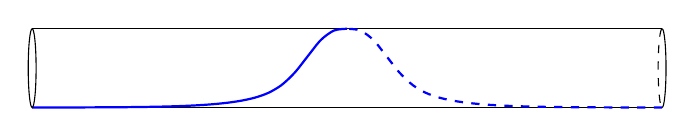
\begin{tikzpicture}[xscale=0.5]
    \draw (-8, 1) -- (8, 1);
    \draw (-8, 0) -- (8, 0);
    \draw [domain=-8:0, thick, blue] plot [smooth] (\x, {exp(-(\x)^2) + (1 - exp(-((\x)^2))) * atan (exp (\x)) / 45});
    \draw [dashed, domain=8:0, thick, blue] plot [smooth] (\x, {exp(-(\x)^2) + (1 - exp(-((\x)^2))) * atan (exp (-\x)) / 45});

    \draw (-8, 0.5) ellipse (0.1 and 0.5);

    \draw (8, 1) arc (90:-90:0.1 and 0.5);
    \draw [dashed] (8, 1) arc (90:270:0.1 and 0.5);
  \end{tikzpicture}
\end{center}
If we view it this way, it is absolutely obvious that no matter how this solution evolves in time, it will never become, or even approach the ``trivial'' solution $u = 0$, even though both satisfy the boundary condition $u \to 0$ as $x \to \pm \infty$.

\subsection{\texorpdfstring{B\"acklund}{Backlund} transformations}
For a linear partial differential equation, we have the principle of superposition --- if we have two solutions, then we can add them to get a third solution. This is no longer true in non-linear PDE's.

One way we can find ourselves a new solution is through a \emph{B\"acklund transformation}. This originally came from geometry, where we wanted to transform a surface to another, but we will only consider the applications to PDE's.

The actual definition of the B\"acklund transformation is complicated. So we start with an example.
\begin{eg}
  Consider the Cauchy-Riemann equation
  \[
    u_x = v_u,\quad u_y = -v_x.
  \]
  We know that the pair $u, v$ satisfies the Cauchy-Riemann equations, if and only if both $u, v$ are harmonic, i.e.\ $u_{xx} + u_{yy} = 0$ etc.

  Now suppose we have managed to find a harmonic function $v = v(x, y)$. Then we can try to solve the Cauchy-Riemann equations, and we would get \emph{another} harmonic function $u = u(x, y)$.

  For example, if $v = 2xy$, then we get the partial differential equations
  \[
    u_x = 2x,\quad u_y = -2y.
  \]
  So we obtain
  \[
    u(x, y) = x^2 - y^2 + C
  \]
  for some constant $C$, and this function $u$ is guaranteed to be a solution to Laplace's equations.

  So the Cauchy-Riemann equation generates new solutions to Laplace's equation from old ones. This is an example of an (auto-)B\"acklund transformation for Laplace's equation.
\end{eg}

In general, we have the following definition:
\begin{defi}[B\"acklund transformation]\index{B\"acklund transformation}
  A \emph{B\"acklund transformation} is a system of equations that relate the solutions of some PDE's to
  \begin{enumerate}
    \item A solution to some other PDE; or
    \item Another solution to the same PDE.
  \end{enumerate}
  In the second case, we call it an \term{auto-B\"acklund transformation}.
\end{defi}

\begin{eg}
  The equation $u_{xt} = e^u$ is related to the equation $v_{xt} = 0$ via the B\"acklund transformation
  \[
    u_x + v_x = \sqrt{2} \exp \left(\frac{u - v}{2}\right),\quad u_t - v_t = \sqrt{2} \exp\left(\frac{u + v}{2}\right).
  \]
  The verification is left as an exercise on the first example sheet. Since $v_{xt} = 0$ is an easier equation to solve, this gives us a method to solve $u_{xt} = e^u$.
\end{eg}

We also have examples of auto-B\"acklund transformations:
\begin{eg}
  For any non-zero constant $\varepsilon$, consider
  \begin{align*}
    \frac{\partial}{\partial \xi}(\varphi_1 - \varphi_2) &= 2 \varepsilon \sin \left(\frac{\varphi_1 + \varphi_2}{2}\right)\\
    \frac{\partial}{\partial \tau}(\varphi_1 + \varphi_2) &= \frac{2}{\varepsilon} \sin\left(\frac{\varphi_1 - \varphi_2}{2}\right).
  \end{align*}
  These equations come from geometry, and we will not go into details motivating these. We can compute
  \begin{align*}
    \frac{\partial^2}{\partial \xi\partial \tau} (\varphi_1 - \varphi_2) &= \frac{\partial}{\partial \tau}\left(2\varepsilon \sin \left(\frac{\varphi_1 + \varphi_2}{2}\right)\right)\\
    &= 2\varepsilon \cos \left(\frac{\varphi_1 + \varphi_2}{2}\right)\frac{\partial}{\partial \tau}\left(\frac{\varphi_1 + \varphi_2}{2}\right)\\
    &= 2 \varepsilon \cos \left(\frac{\varphi_1 + \varphi_2}{2}\right) \frac{1}{2} \cdot \frac{2}{\varepsilon} \sin \left(\frac{\varphi_1 - \varphi_2}{2}\right)\\
    &= 2 \cos \left(\frac{\varphi_1 + \varphi_2}{2}\right)\sin \left(\frac{\varphi_1 - \varphi_2}{2}\right)\\
    &= \sin \varphi_1 - \sin \varphi_2.
  \end{align*}
  It then follows that
  \[
    \frac{\partial^2 \varphi_2}{\partial \xi \partial \tau} = \sin \varphi_2\quad\Longleftrightarrow\quad \frac{\partial^2 \varphi_1}{\partial \xi \partial \tau} = \sin \varphi_1.
  \]
  In other words, $\varphi_1$ solves the sine-Gordon equations in light cone coordinates, if and only if $\varphi_2$ does. So this gives an auto-B\"acklund transformation for the sine-Gordon equation. Moreover, since we had a free parameter $\varepsilon$, we actually have a \emph{family} of auto-B\"acklund transforms.

  For example, we already know a solution to the sine-Gordon equation, namely $\varphi_1 = 0$. Using this, the equations say we need to solve
  \begin{align*}
    \frac{\partial \varphi}{\partial \xi} &= 2\varepsilon \sin \frac{\varphi}{2}\\
    \frac{\partial \varphi}{\partial \tau} &= -\frac{2}{\varepsilon} \sin \frac{\varphi}{2}.
  \end{align*}
  We see this equation has some sort of symmetry between $\xi$ and $\tau$. So we use an ansatz
  \[
    \varphi(\xi, \tau) = 2\chi (\varepsilon \xi - \varepsilon^{-1} \tau).
  \]
  Then both equations tell us
  \[
    \frac{\d \chi}{\d x} = \sin \chi.
  \]
  We can separate this into
  \[
    \csc \chi \;\d \chi = \d x.
  \]
  Integrating this gives us
  \[
    \log \tan \frac{\chi}{2} = x + C.
  \]
  So we find
  \[
    \chi(x) = 2\tan^{-1} (Ae^x).
  \]
  So it follows that
  \[
    \varphi(\xi, \tau) = 2 \tan^{-1} (A (\varepsilon \xi + \varepsilon^{-1}\tau)),
  \]
  where $A$ and $\varepsilon$ are free parameters. After a bit more work, this was the 1-soliton solution we previously found.

  Applying the B\"acklund transform again to this new solution produces multi-soliton solutions.
\end{eg}

\section{Inverse scattering transform}
Recall that in IB Methods, we decided we can use Fourier transforms to solve PDE's. For example, if we wanted to solve the Klein--Gordon equation
\[
  u_{tt} - u_{xx} = u,
\]
then we simply had to take the Fourier transform with respect to $x$ to get
\[
  \hat{u}_{tt} + k^2 \hat{u} = \hat{u}.
\]
This then becomes a very easy ODE in $t$:
\[
  \hat{u}_{tt} = (1 - k^2) \hat{u},
\]
which we can solve. After solving for this, we can take the inverse Fourier transform to get $u$.

The inverse scattering transform will follow a similar procedure, except it is much more involved and magical. Again, given a differential equation in $u(x, t)$, for each fixed time $t$, we can transform the solution $u(x, t)$ to something known as the \emph{scattering data} of $u$. Then the differential equation will tell us how the scattering data should evolve. After we solved for the scattering data at all times, we invert the transformation and recover the solution $u$.

We will find that each step of that process will be linear, i.e.\ easy, and this will magically allow us to solve non-linear equations.
\subsection{Forward scattering problem}
\index{forward scattering problem}
Before we talk about the inverse scattering transform, it is helpful to know what the \emph{forward} problem is. This is, as you would have obviously guessed, related to the Schr\"odinger operator we know and love from quantum mechanics. Throughout this section, $L$ will be the Schr\"odinger operator
\[
  L = -\frac{\partial^2}{\partial x^2} + u(x),
\]
where the ``potential'' $u$ has compact support, i.e.\ $u = 0$ for $|x|$ sufficiently large. What we actually need is just that $u$ decays quickly enough as $|x| \to \infty$, but to make our life easy, we do not figure out the precise conditions to make things work, and just assume that $u$ actually vanishes for large $|x|$. For a fixed $u$, we are interested in an eigenvalue (or ``spectral'') problem, i.e.\ we want to find solutions to
\[
  L \psi = \lambda \psi.
\]
This is the ``forward'' problem, i.e.\ given a $u$, we want to find the eigenvalues and eigenfunctions. The \emph{inverse} problem is given the collection of all such eigenvalues and eigenfunctions, some sort of solutions like this, we want to find out what $u$ is.

We will divide this into the continuous and discrete cases.
\subsubsection{Continuous spectrum}\label{sssec:continuous-spectrum}
Here we consider solutions to $L\psi = k^2 \psi$ for real $k$. Since $u = 0$ for $|x|$ large, we must have
\[
  \psi_{xx} + k^2 \psi = 0
\]
for large $|x|$.

So solutions as $|x| \to \infty$ are linear combinations of $e^{\pm i k x}$. We look for specific solutions for $\psi = \varphi(x, k)$ defined by the condition
\[
  \varphi = e^{-ikx}\text{ as } x \to -\infty.
\]
Then there must be coefficients $a = a(k)$ and $b = b(k)$ such that
\[
  \phi(x, k) = a(k) e^{-ikx} + b(k) e^{ikx}\text{ as }x \to +\infty.
\]
We define the quantities
\[
  \Phi(x, k) = \frac{\varphi(x, k)}{a(k)},\quad R(k) = \frac{b(k)}{a(k)},\quad T(k) = \frac{1}{a(k)}.
\]
Here $R(k)$ is called the \term{reflection coefficient}, and $A(k)$ is the \term{transmission coefficient}. You may have seen these terms from IB Quantum Mechanics. Then we can write
\[
  \Phi(x, k) =
  \begin{cases}
    T(k) e^{-ikx} & x \to -\infty\\
    e^{-ikx} + R(k) e^{kx} & x \to +\infty
  \end{cases}.
\]
We can view the $e^{-ikx}$ term as waves travelling to the left, and $e^{ikx}$ as waves travelling to the right. Thus in this scenario, we have an incident $e^{-ikx}$ wave coming from the right, the potential reflects some portion of the wave, namely $R(k) e^{ikx}$, and transmits the remaining $T(k) e^{-ikx}$. It will be shown on the first example sheet that in fact $|T(k)|^2 + |R(k)|^2 = 1$.

What would happen when we change $k$? Since $k$ is the ``frequency'' of the wave, which is proportional to the energy we would expect that the larger $k$ is, the more of the wave is transmitted. Thus we might expect that $T(k) \to 1$, and $R(k) \to 0$. This is indeed true, but we will not prove it. We can think of these as ``boundary conditions'' for $T$ and $R$.

So far, we've only been arguing hypothetically about what the solution has to look like if it existed. However, we do not know if there is a solution at all!

In general, differential equations are bad. They are hard to talk about, because if we differentiate a function, it generally gets worse. It might cease to be differentiable, or even continuous. This means differential operators could take our function out of the relevant function space we are talking about. On the other hand, integration makes functions look \emph{better}. The more times we integrate, the smoother it becomes. So if we want to talk about the existence of solutions, it is wise to rewrite the differential equation as an integral solution instead.

We consider the integral equation for $f = f(x, k)$ given by
\[
  f(x, k) = f_0(x, k) + \int_{-\infty}^\infty G(x - y, k) u(y) f(y, k) \;\d y,
\]
where $f_0$ is any solution to $(\partial^2_x + k^2) f_0 = 0$, and $G$ is the Green's function for the differential operator $\partial^2_x + k^2$, i.e.\ we have
\[
  (\partial_x^2 + k^2) G = \delta(x).
\]
What we want to show is that if we can find an $f$ that satisfies this integral equation, then it also satisfies the eigenvalue equation. We simply compute
\begin{align*}
  (\partial_x^2 + k^2) f &= (\partial_x^2 + k^2)f_0 + \int_{-\infty}^\infty (\partial_x^2 + k^2) G(x - y, k) u(y) f(y, k) \;\d y\\\
  &= 0 + \int_{-\infty}^\infty \delta(x - y) u(y) f(y, k)\;\d y\\
  &= u(x) f(x, k).
\end{align*}
In other words, we have
\[
  Lf = k^2 f.
\]
So it remains to prove that solutions to the integral equation exists.

We pick $f_0 = e^{-ikx}$ and
\[
  G(x, k) =
  \begin{cases}
    0 & x < 0\\
    \frac{1}{k} \sin (kx) & x \geq 0
  \end{cases}.
\]
Then our integral equation automatically implies
\[
  f(x, k) = e^{-ikx}
\]
as $x \to -\infty$, because for very small $x$, either $x - y < 0$ or $y$ is very small, so the integral always vanishes as $u$ has compact support.

To solve the integral equation, we write this in abstract form
\[
  (I - K) f = f_0,
\]
where $I$ is the identity, and
\[
  (Kf)(x) = \int_{-\infty}^\infty G(x - y, k) u(y) f(y, k) \;\d y.
\]
So we can ``invert''
\[
  f = (I - K)^{-1} f_0.
\]
We can ``guess'' a solution to the inverse. If we don't care about rigour and just expand this, we get
\[
  f = (I + K + K^2 + \cdots)f_0.
\]
It doesn't matter how unrigorous our derivation was. To see it is a valid solution, we just have to check that it works! The first question to ask is if this expression converges. On the second example sheet, we will show that this thing actually converges. If this holds, then we have
\[
  (I - K)f = If_0 + K f_0 + K^2 f_0 + \cdots - (K + K^2 f_0 + K^3 f_0 + \cdots) = f_0.
\]
So this is a solution!

Of course, this result is purely formal. Usually, there are better \emph{ad hoc} ways to solve the equation, as we know from IB Quantum Mechanics.

\subsubsection{Discrete spacetime and bound states}
We now consider the case $\lambda = - \kappa^2 < 0$, where we wlog $\lambda > 0$. We are going to seek solutions to
\[
  L \psi_\kappa = - \kappa^2 \psi_\kappa.
\]
This time, we are going to ask that
\[
  \|\psi_\kappa\|^2 = \int_{-\infty}^\infty \psi_\kappa(x)^2 \;\d x = 1.
\]
We will wlog $\psi_\kappa \in \R$. We will call these things \term{bound states}.

Since $u$ has compact support, any solution
\[
  L \varphi = - \kappa^2 \varphi
\]
must obey
\[
  \varphi_{xx} - \kappa^2 \phi = 0
\]
for $|x| \to \infty$. Then the solutions are linear combinations of $e^{\pm \kappa x}$ as $|x| \to \infty$. We now fix $\varphi_\kappa$ by the boundary condition
\[
  \varphi_\kappa(x) = e^{-\kappa x} \text{ as } x \to +\infty
\]
Then as $x \to -\infty$, there must exist coefficients $\alpha = \alpha(\kappa)$, $\beta = \beta(\kappa)$ such that
\[
  \varphi_\kappa(x) = \alpha(\kappa) e^{\kappa x} + \beta(\kappa) e^{-\kappa x}\text{ as }x \to -\infty.
\]
Note that for \emph{any} $\kappa$, we can solve the equation $L \varphi = - \kappa^2 \varphi$ and find a solution of this form. However, we have the additional condition that $\|\psi_\kappa\|^2 = 1$, and in particular is finite. So we must have $\beta(\kappa) = 0$. It can be shown that the function $\beta = \beta(\kappa)$ has only finitely many zeroes
\[
  \chi_1 > \chi_2 > \cdots > \chi_N > 0.
\]
%To show this, we will have to find out an explicit expression for the solution of $\varphi_\kappa$, just as we did for the continuous spectrum, and then explicitly find a formula of $\beta$. We can then find that it has finitely many zeros.
So we have a finite list of bound-states $\{\psi_n\}_{n= 1}^N$, written
\[
  \psi_n(x) = c_n \varphi_{\chi_n}(x),
\]
where $c_n$ are normalization constants chosen so that $\|\psi_n\| = 1$.

\subsubsection{Summary of forward scattering problem}
In summary, we had a spectral problem
\[
  L\psi = \lambda \psi,
\]
where
\[
  L = -\frac{\partial^2}{\partial x^2} + u,
\]
where $u$ has compact support. The goal is to find $\psi$ and $\lambda$.

In the continuous spectrum, we have $\lambda = k^2 > 0$. Then we can find some $T(k)$ and $R(k)$ such that
\[
  \phi(x, k) =
  \begin{cases}
    T(k) e^{-ikx} & x \to -\infty\\
    e^{-ikx} + R(k) e^{kx} & x \to +\infty
  \end{cases},
\]
and solutions exist for all $k$.

In the discrete spectrum, we have $\lambda = - \kappa^2 < 0$. We can construct \emph{bound states} $\{\psi_n\}_{n = 1}^N$ such that $L\psi_n = - \chi_n^2 \psi_n$ with
\[
  \chi_1 > \chi_2 > \cdots > \chi_N > 0,
\]
and $\|\psi_n\| = 1$.

Bound states are characterized by large, positive $x$ behaviour
\[
  \psi_n(x) = c_n e^{-\chi_n x}\text{ as }x \to +\infty,
\]
where $\{c_n\}_{n = 1}^N$ are normalization constants.

Putting all these together, the \term{scattering data} for $L$ is
\[
  S = \left\{\{\chi_n, c_n\}_{n = 1}^N, R(k), T(k)\right\}.
\]
\begin{eg}
  Consider the Dirac potential $u(x) = - 2 \alpha \delta(x)$, where $\alpha > 0$. Let's try to compute the scattering data.

  We do the continuous spectrum first. Since $u(x) = 0$ for $x \not= 0$, we must have
  \[
    \Phi(x, k) =
    \begin{cases}
      T(k) e^{-ikx} & x < 0\\
      e^{-ikx} + R(k) e^{ikx} & x > 0
    \end{cases}
  \]
  Also, we want $\Phi(x, k)$ to be continuous at $x = 0$. So we must have
  \[
    T(k) = 1 + R(k).
  \]
  By integrating $L\Phi = k^2 \Phi$ over $(-\varepsilon, \varepsilon)$, taking $\varepsilon \to 0$, we find that $\frac{\partial \Phi}{\partial x}$ has a jump discontinuity at $x = 0$ given by
  \[
    ik(R - 1) + ikT = -2 \alpha T.
  \]
  We now have two equations and two unknowns, and we can solve to obtain
  \[
    R(k) = \frac{i\alpha}{k - i\alpha},\quad T(k) = \frac{k}{k - i \alpha}.
  \]
  We can see that we indeed have
  \[
    |R|^2 + |T|^2 = 1.
  \]
  Note that as $k$ increases, we find that $R(k) \to 0$ and $T(k) \to 1$. This makes sense, since we can think of $k$ as the energy of the wave, and the larger the energy, the more likely we are to pass through.

  Now let's do the discrete part of the spectrum, and we jump through the same hoops. Since $\delta(x) = 0$ for $x \not= 0$, we must have
  \[
    -\frac{\partial^2 \psi_n}{\partial x^2} + \chi_n^2 \psi_n = 0
  \]
  for $x \not= 0$. So we have
  \[
    \psi_n(x) = c_n e^{- \chi_n |x|}.
  \]
  Integrating $L\psi_n = - \chi_n^2 \psi_n$ over $(-\varepsilon, \varepsilon)$, we similarly find that
  \[
    c_n \chi_n = c_n \alpha.
  \]
  So there is just one bound state, with $\chi_1 = \alpha$. We finally find $c_n$ by requiring $\norm{\psi_1} = 1$. We have
  \[
    1 = \int_{-\infty}^\infty \psi_1(x)^2 \;\d x = c_1^2 \int_{-\infty}^\infty e^{-2 \chi_1|x|}\;\d x = \frac{c_1^2}{\alpha}.
  \]
  So we have
  \[
    c_1 = \sqrt{\alpha}.
  \]
  In total, we have the following scattering data:
  \[
    S = \left\{\{\alpha, \sqrt{\alpha}\},\quad \frac{i\alpha}{k - i \alpha},\quad \frac{k}{k - i\alpha}\right\}.
  \]
\end{eg}

\subsection{Inverse scattering problem}
We might be interested in the inverse problem. Given scattering data
\[
  S = \left\{\{\chi_n, c_n\}_{n = 1}^N, R(k), T(k)\right\},
\]
can we reconstruct the potential $u = u(x)$ such that
\[
  L = -\frac{\partial^2}{\partial x^2} + u(x)
\]
has scattering data $S$? The answer is yes! Moreover, it turns out that $T(k)$ is not needed.

We shall write down a rather explicit formula for the inverse scattering problem, but we will not justify it.
\begin{thm}[GLM inverse scattering theorem]\index{GLM inverse scattering theorem}
  A potential $u = u(x)$ that decays rapidly to $0$ as $|x| \to \infty$ is completely determined by its scattering data
  \[
    S = \left\{\{\chi_n, c_n\}_{n = 1}^N, R(k)\right\}.
  \]
  Given such a scattering data, if we set
  \[
    F(x) = \sum_{n = 1}^N c_n^2 e^{-\chi_n x} + \frac{1}{2\pi} \int_{-\infty}^\infty e^{ikx} R(k) \;\d k,
  \]
  and define $k(x, y)$ to be the \emph{unique} solution to
  \[
    k(x, y) + F(x + y) + \int_{x}^\infty k(x, z) f(z + y) \;\d z = 0,
  \]
  then
  \[
    u(x) = -2 \frac{\d}{\d x} k(x, x).
  \]
\end{thm}

\begin{proof}
  Too hard.
\end{proof}
Note that this equation
\[
  k(x, y) + F(x + y) + \int_{x}^\infty k(x, z) f(z + y) \;\d z = 0
\]
is not too hard to solve. We can view it as a linear equation of the form
\[
  \mathbf{x} + \mathbf{b} + A \mathbf{x} = 0
\]
for some linear operator $A$, then use our familiar linear algebra techniques to guess a solution. Afterwards, we can then verify that it works. We will see an explicit example later on when we actually use this to solve problems.

Now that we've got this result, we understand how scattering problems work. We know how to go forwards \emph{and} backwards.

This is all old theory, and not too exciting. The real exciting thing is how we are going to use this to solve PDE's. Given the KdV equation
\[
  u_t + u_{xxx} - 6uu_x = 0,
\]
we can think of this as a potential evolving over time, with a starting potential $u(x, 0) = u_0(x)$. We then compute the initial scattering data $T$, $R$, $\chi$ and $c$. Afterwards, we obtain the corresponding equations of evolution of the scattering data form the KdV equation. It turns out this is really simple --- the $\chi_n$ are always fixed, and the others evolve as
\begin{align*}
  R(k, t) &= e^{8ik^3 t}R(k, 0)\\
  T(k, t) &= T(k, 0)\\
  c_n(t) &=e^{4 \chi_n^3 t} c_n(0).
\end{align*}
Then we use this GLM formula to reconstruct the potential $u$ at all times!

\subsection{Lax pairs}
The final ingredient to using the inverse scattering transform is how to relate the evolution of the potential to the evolution of the scattering data. This is given by a \emph{lax pair}.

Recall that when we studied Hamiltonian systems at the beginning of the course, under a Hamiltonian flow, functions evolve by
\[
  \frac{\d f}{\d t} = \{f, H\}.
\]
In quantum mechanics, when we ``quantize'' this, in the Heisenberg picture, the operators evolve by
\[
  i\hbar \frac{\d L}{\d t} = [L, H].
\]
In some sense, these equations tell us $H$ ``generates'' time evolution. What we need here is something similar --- an operator that generates the time evolution of our operator.
\begin{defi}[Lax pair]\index{Lax pair}
  Consider a time-dependent self-adjoint linear operator
  \[
    L = a_m (x, t) \frac{\partial^m}{\partial x^m} + \cdots + a_1 (x, t) \frac{\partial}{\partial x} + a_0(x, t),
  \]
  where the $\{a_i\}$ (possibly matrix-valued) functions of $(x, t)$. If there is a second operator $A$ such that
  \[
    L_t = LA - AL = [L, A],
  \]
  where
  \[
    L_t = \dot{a}_m \frac{\partial^m}{\partial x^m} + \cdots + \dot{a}_0,
  \]
  denotes the derivative of $L$ with respect to $t$, then we call $(L, A)$ a \emph{Lax pair}.
\end{defi}

The main theorem about Lax pairs is the following isospectral flow theorem:
\begin{thm}[Isospectral flow theorem]\index{isospectral flow theorem}
  Let $(L, A)$ be a Lax pair. Then the discrete eigenvalues of $L$ are time-independent. Also, if $L\psi = \lambda \psi$, where $\lambda$ is a discrete eigenvalue, then
  \[
    L \tilde{\psi} = \lambda \tilde{\psi},
  \]
  where
  \[
    \tilde{\psi} = \psi_t + A \psi.
  \]
\end{thm}
The word ``isospectral'' means that we have an evolving system, but the eigenvalues are time-independent.

\begin{proof}
  We will assume that the eigenvalues at least vary smoothly with $t$, so that for each eigenvalue $\lambda_0$ at $t = 0$ with eigenfunction $\psi_0(x)$, we can find some $\lambda(t)$ and $\psi(x, t)$ with $\lambda(0) = \lambda_0$, $\psi(x, 0) = \psi_0(x)$ such that
  \[
    L(t) \psi(x, t) = \lambda(t) \psi (x, t).
  \]
  We will show that in fact $\lambda(t)$ is constant in time. Differentiating with respect to $t$ and rearranging, we get
  \begin{align*}
    \lambda_t \psi &= L_t \psi + L \psi_t - \lambda \psi_t\\
    &= LA \psi - AL \psi + L \psi_t - \lambda \psi_t\\
    &= LA \psi - \lambda A \psi + L \psi_t - \lambda \psi_t\\
    &= (L - \lambda)(\psi_t + A \psi)
  \end{align*}
  We now take the inner product $\psi$, and use that $\|\psi\| = 1$. We then have
  \begin{align*}
    \lambda_t &= \bra \psi, \lambda_t \psi\ket\\
    &= \bra \psi, (L - \lambda)(\psi_t + A_\psi)\ket\\
    &= \bra (L - \lambda)\psi, \psi_t + A_\psi\ket\\
    &= 0,
  \end{align*}
  using the fact that $L$, hence $L - \lambda$ is self-adjoint.

  So we know that $\lambda_t = 0$, i.e.\ that $\lambda$ is time-independent. Then our above equation gives
  \[
    L \tilde{\psi} = \lambda \tilde{\psi},
  \]
  where
  \[
    \tilde{\psi} = \psi_t + A\psi.\qedhere
  \]
\end{proof}

In the case where $L$ is the Schr\"odinger operator, the isospectral theorem tells us how we can relate the evolution of some of the scattering data (namely the $\chi_n$), to some differential equation in $L$ (namely the Laxness of $L$). For a cleverly chosen $A$, we will be able to relate the Laxness of $L$ to some differential equation in $u$, and this establishes our first correspondence between evolution of $u$ and the evolution of scattering data.
\begin{eg}
  Consider
  \begin{align*}
    L &= -\partial_x^2 + u(x, t)\\
    A &= 4 \partial_x^3 - 3 (u \partial_x + \partial_x u).
  \end{align*}
  Then $(L, A)$ is a Lax pair iff $u = u(x, t)$ satisfies KdV. In other words, we have
  \[
    L_t - [L, A] = 0 \quad\Longleftrightarrow\quad u_t + u_{xxx} - 6uu_x =0 .
  \]
\end{eg}

\subsection{Evolution of scattering data}
Now we do the clever bit: we allow the potential $u = u(x, t)$ to evolve via KdV
\[
  u_t + u_{xxx} - 6 u u_x = 0.
\]
We see how the scattering data for $L = -\partial_x^2 + u(x, t)$ evolves. Again, we will assume that $u$ has compact support. Note that this implies that we have
\[
  A = 4 \partial_x^3\text{ as }|x| \to \infty.
\]
\subsubsection{Continuous spectrum (\tph{$\lambda = k^2 > 0$}{lambda = k2 > 0}{&lambda; = k<sup>2</sup> &gt; 0})}
As in Section \ref{sssec:continuous-spectrum}, for each $t$, we can construct a solution $\varphi$ to $L \varphi = k^2 \varphi$ such that
\[
  \varphi(x, t) =
  \begin{cases}
    e^{-ikx} & x \to -\infty\\
    a(k, t) e^{-ikx} + b(k, t) e^{ikx} & x \to \infty
  \end{cases}.
\]
This time, we know that for any $u$, we can find a solution for any $k$. So we can assume that $k$ is fixed in the equation
\[
  L\varphi = k^2 \varphi.
\]
We assume that $u$ is a solution to the KdV equation, so that $(L, A)$ is a Lax pair. As in the proof of the isospectral flow theorem, we differentiate this to get
\[
  0 = (L - k^2)(\varphi_t + A_\varphi).
\]
This tells us that
\[
  \tilde{\varphi} = \varphi_t + A \varphi
\]
solves
\[
  L \tilde{\varphi} = k^2 \tilde{\varphi}.
\]
We can try to figure out what $\tilde{\varphi}$ is for large $|x|$. We recall that for large $|x|$, we simply have $A = 4 \partial_x^3$. Then we can write
\[
  \tilde{\varphi}(x, t) =
  \begin{cases}
    4 ik^3 e^{-ikx} & x \to -\infty\\
    (a_t + 4 ik^3 a)e^{-ikx} + (b_t - 4ik^3 b) e^{ikx} & x \to \infty
  \end{cases}
\]
We now consider the function
\[
  \theta = 4ik^3 \varphi - \tilde{\varphi}.
\]
By linearity of $L$, we have
\[
  L \theta = k^2 \theta.
\]
Note that by construction, we have $\theta(x, t) \to 0$ as $x \to -\infty$. We recall that the solution to $Lf = k^2 f$ for $f = f_0$ as $x \to -\infty$ is just
\begin{align*}
  f &= (I - K)^{-1} f_0\\
  &= (I + K + K^2 + \cdots)f_0
\end{align*}
So we obtain
\[
  \theta = (1 + K + K^2 + \cdots) 0 = 0.
\]
So we must have
\[
  \tilde{\varphi} = 4ik^3 \varphi.
\]
Looking at the $x \to +\infty$ behaviour, we figure that
\begin{align*}
  a_t + 4ik^3 a &= 4 ik^3 a\\
  b_t - 4ik^3 b &= 4ik^3 b
\end{align*}
Of course, these are equations we can solve. We have
\begin{align*}
  a(k, t) &= a(k, 0)\\
  b(k, t) &= b(k, 0) e^{8ik^3 t}.
\end{align*}
In terms of the reflection and transmission coefficients, we have
\begin{align*}
  R(k, t) &= R(k, 0) e^{8ik^3 t}\\
  T(k, t) &= T(k, 0).
\end{align*}
Thus, we have shown that if we assume $u$ evolves according to the \emph{really} complicated KdV equation, then the scattering data must evolve in this simple way! This is \emph{AMAZING}.

\subsubsection{Discrete spectrum (\tph{$\lambda= -\kappa^2 < 0$}{lambda = -kappa^2 < 0}{&labmda; = -&kappa;<sup>2</sup> &lt; 0})}
The discrete part is similar. By the isospectral flow theorem, we know the $\chi_n$ are constant in time. For each $t$, we can construct bound states $\{\psi_n(x, t)\}_{n = 1}^N$ such that
\[
  L\psi_n = - \chi_n^2 \psi_n,\quad \|\psi_n\| = 1.
\]
Moreover, we have
\[
  \psi_n(x, t) = c_n(t) e^{-\chi_n|x|} \text{ as }x \to +\infty.
\]
From the isospectral theorem, we know the function
\[
  \tilde{\psi}_n = \partial_t \psi_n + A\psi_n
\]
also satisfies
\[
  L\tilde{\psi}_n = - \chi_n^2 \tilde{\psi}_n
\]
It is an exercise to show that these solutions must actually be proportional to one another. Looking at Wronskians, we can show that $\tilde{\psi}_n \propto \psi_n$. Also, we have
\begin{align*}
  \bra \psi_n, \tilde{\psi}_n\ket &= \bra \psi_n, \partial_t \psi_n\ket + \bra\psi_n, A \psi_n\ket\\
  &= \frac{1}{2} \frac{\partial}{\partial t} \bra \psi_n, \psi_n\ket + \bra \psi_n, A \psi_n\ket\\
  &= 0,
\end{align*}
using the fact that $A$ is antisymmetric and $\|\psi_n\|$ is constant. We thus deduce that $\tilde{\psi}_n = 0$.

Looking at large $x$-behaviour, we have
\[
  \tilde{\psi}_n(x, t) = (\dot{c}_n - 4 \chi_n^3 c_n) e^{- \chi_n x}
\]
as $x \to +\infty$. Since $\tilde{\psi}_n \equiv 0$, we must have
\[
  \dot{c}_n - 4 \chi_n^3 c_n = 0.
\]
So we have
\[
  c_n(t) = c_n(0) e^{4 \chi_n^3 t}.
\]
This is again \emph{AMAZING}.

\subsubsection{Summary of inverse scattering transform}
So in summary, suppose we are given that $u = u(x, t)$ evolves according to KdV, namely
\[
  u_t + u_{xxx} - 6uu_x = 0.
\]
If we have an initial condition $u_0(x) = u(x, 0)$, then we can compute its scattering data
\[
  S(0) = \left\{\{\chi_n, c_n(0)\}_{n = 1}^N, R(k, 0)\right\}.
\]
Then for arbitrary time, the scattering data for $L = -\partial_x^2 + u$ is
\[
  S(t) = \left\{\{\chi_n, c_n(0)e^{4\chi_n^3 t}\}_{n = 1}^N, R(k, 0)e^{8ik^3 t}\right\}.
\]
We then apply GLM to obtain $u(x, t)$ for all time $t$.
\[
  \begin{tikzcd}[row sep=5em, column sep=8em]
    u_0(x) \ar[r, "\text{Construct scattering data}", "L = -\partial_x^2 + u_0(x)"'] \ar[d, "\substack{\text{KdV}\\\text{equation}}"] & S(0) = \left\{\{\chi_n, c_n(0)\}_{n = 1}^N, R(k, 0)\right\} \ar[d, "\substack{\text{Evolve}\\\text{scattering}\\\text{data}}"', "{L_t = [L, A]}"]\\
    u(x, t) & S(t) = \left\{\{\chi_n, c_n(0)e^{4\chi_n^3 t}\}_{n = 1}^N, R(k, 0)e^{8ik^3 t}\right\} \ar[l, "\text{Solve GLM equation}"]
  \end{tikzcd}
\]
The key thing that makes this work is that $u_t + u_{xxx} - 6 uu_x$ holds if and only if $L_t = [L, A]$.

For comparison, this is what we would do if we had to solve $u_t + u_{xxx} = 0$ by a Fourier transform:
\[
  \begin{tikzcd}[row sep=5em, column sep=8em]
    u_0(x) \ar[r, "\text{Fourier transform}"] \ar[d, "u_t + u_{xxx} = 0"] & \hat{u}_0(k) \ar[d, "\hat{u}_t - ik^3 \hat{u} = 0"]\\
    u(x, t) & \hat{u}(u, t) = \hat{u}_0(k) e^{ik^3 t} \ar[l, "\text{Inverse Fourier}"', "\text{Transform}"]
  \end{tikzcd}
\]
It is just the same steps, but with a simpler transform!

\subsection{Reflectionless potentials}
We are now going to actually solve the KdV equation for a special kind of potential --- reflectionless potentials.

\begin{defi}[Reflectionless potential]\index{reflectionless potential}\index{potential!reflectionless}
  A \emph{reflectionless potential} is a potential $u(x, 0)$ satisfying $R(k, 0) = 0$.
\end{defi}

Now if $u$ evolves according to the KdV equation, then
\[
  R(k, t) = R(k, 0) e^{8ik^3 t} = 0.
\]
So if a potential starts off reflectionless, then it remains reflectionless.

We now want to solve the GLM equation in this case. Using the notation when we wrote down the GLM equation, we simply have
\[
  F(x) = \sum_{n = 1}^N c_n^2 e^{-\chi_n x}.
\]
We will mostly not write out the $t$ when we do this, and only put it back in at the very end. We now guess that the GLM equation has a solution of the form
\[
  K(x, y) = \sum_{m = 1}^N K_m(x) e^{-\chi_m y}
\]
for some unknown functions $\{K_m\}$ (in the second example sheet, we show that it \emph{must} have this form). We substitute this into the GLM equation and find that
\[
  \sum_{n = 1}^N \left[c_n^2 e^{-\chi_n x}+ K_n(x) + \sum_{m = 1}^N c_n^2 K_m(x) \int_x^\infty e^{-(\chi_n + \chi_m)z}\;\d z\right] e^{-\chi_n y} = 0.
\]
Now notice that the $e^{-\chi_n y}$ for $n = 1, \cdots, N$ are linearly independent. So we actually have $N$ equations, one for each $n$. So we know that
\[
  c_n^2 e^{-\chi_n x} + K_n(x) + \sum_{m = 1}^N \frac{c_n^2 K_m(x)}{\chi_n + \chi_m} e^{-(\chi_n + \chi_m)x} = 0\tag{$*$}
\]
for all $n = 1, \cdots, N$. Now if our goal is to solve the $K_n(x)$, then this is just a linear equation for each $x$! We set
\begin{align*}
  \mathbf{c} &= (c_1^2 e^{-\chi_1 x}, \cdots, c_N^2 e^{-\chi_N x})^T\\
  \mathbf{K} &= (K_1(x), \cdots, K_N(x))^T\\
  A_{nm} &= \delta_{nm} + \frac{c_n^2 e^{-(\chi_n - \chi_m)x}}{\chi_n + \chi_m}.
\end{align*}
Then $(*)$ becomes
\[
  A\mathbf{K} = -\mathbf{c}.
\]
This really is a linear algebra problem. But we don't really have to solve this. The thing we really want to know is
\begin{align*}
  K(x, x) &= \sum_{m = 1}^N K_m(x) e^{-\chi_m x}\\
  &= \sum_{m = 1}^N \sum_{m = 1}^N (A^{-1})_{mn} (-\mathbf{c})_n e^{-\chi_m x}
\end{align*}
Now note that
\[
  \frac{\d}{\d x}A_{nm}(x) = A_{nm}'(x) = - c_n^2 e^{-\chi_n x} e^{-\chi_m x} = (-\mathbf{c})_n e^{-\chi_m x}.
\]
So we can replace the above thing by
\[
  K(x, x) = \sum_{m = 1}^N \sum_{n = 1}^N (A^{-1})_{mn} A'_{nm} = \tr(A^{-1}A').
\]
It is an exercise on the second example sheet to show that this is equal to
\[
  K(x, x) = \frac{1}{\det A} \frac{\d}{\d x} (\det A) = \frac{\d}{\d x} \log (\det A).
\]
So we have
\[
  u(x) = - 2 \frac{\d^2}{\d x^2} \log(\det A).
\]
We now put back the $t$-dependence we didn't bother to write all along. Then we have
\[
  u(x, t) = -2 \frac{\partial^2}{\partial x^2} \log(\det A(x, t)),
\]
where
\[
  A_{nm}(x, t) = \delta_{nm} + \frac{c_n(0)^2 e^{8\chi_n^3 t}e^{-(\chi_n + \chi_m)x}}{\chi_n + \chi_m}.
\]
It turns out these are soliton solutions, and the number of discrete eigenstates $N$ is just the number of solitons!
\subsection{Infinitely many first integrals}
As we've previously mentioned, we are expecting our integrable PDE's to have infinitely many first integrals. Recall we can construct $\varphi = \varphi(x, k, t)$ such that
\[
  L\varphi = k^2 \varphi,
\]
and we had
\[
  \varphi(x, k, t) =
  \begin{cases}
    e^{-ikx} & x \to -\infty\\
    a(k, t) e^{-ikx} + b(k, t) e^{ikx} & x \to \infty
  \end{cases}.
\]
But when we looked at the evolution of the scattering data, we can actually write down what $a$ and $b$ are. In particular, $a(k, t) = a(k)$ is independent of $t$. So we might be able to extract some first integrals from it. We have
\[
  e^{ikx} \varphi(x, k, t) = a(k) + b(k, t) e^{2ikx} \text{ as }x \to \infty.
\]
We now take the average over $[R, 2R]$ for $R \to \infty$. We do the terms one by one. We have the boring integral
\[
  \frac{1}{R} \int_R^{2R} a(k) \;\d x = a(k).
\]
For the $b(k, t)$ term, we have
\[
  \frac{1}{R} \int_R^{2R} b(k, t) e^{2ikx} \;\d x = O\left(\frac{1}{R}\right),
\]
So we have
\begin{align*}
  a(k) &= \lim_{R \to \infty} \frac{1}{R} \int_R^{2R} e^{ikx} \varphi(x, k, t) \;\d x\\
  &= \lim_{R \to \infty} \int_1^2 e^{ikRx} \varphi(Rx, k, t) \;\d x.
\end{align*}
So can we figure out what this thing is? Since $\varphi = e^{-ikx}$ as $x \to -\infty$, it is ``reasonable'' to write
\[
  \varphi(x, k, t) = \exp\left(-ikx + \int_{-\infty}^x S(y, k, t)\;\d y\right)
\]
for some function $S$. Then after some dubious manipulations, we would get
\begin{align*}
  a(k) &= \lim_{R \to \infty} \int_1^2 \exp\left(\int_{-\infty}^{Rx} S(y, k, t)\;\d y\right)\;\d x\\
  &= \exp\left(\int_{-\infty}^\infty S(y, k, t)\;\d y\right).\tag{$\dagger$}
\end{align*}
Now this is interesting, since the left hand side $a(k)$ has no $t$-dependence, but the right-hand formula does. So this is where we get our first integrals from.

Now we need to figure out what $S$ is. To find $S$, recall that $\varphi$ satisfies
\[
  L\varphi = k^2 \varphi.
\]
So we just try to shove our formula of $\varphi$ into this equation. Notice that
\[
  \varphi_x = (S - ik) \varphi,\quad \varphi_{xx} = S_x \varphi + (S - ik)^2 \varphi.
\]
We then put these into the Schr\"odinger equation to find
\[
  S_x - (2ik)S + S^2 = -u.
\]
We have got no $\varphi$'s left. This is a famous type of equation --- a \term{Ricatti-type equation}. We can make a guess
\[
  S(x, k, t) = \sum_{n = 1}^\infty \frac{S_n(x, t)}{(2ik)^n}.
\]
This seems like a strange thing to guess, but there are indeed some good reasons for this we will not get into. Putting this into the equation and comparing coefficients of $k^{-n}$, we obtain a recurrence relation
\begin{align*}
  S_1 &= -u\\
  S_{n + 1} &= \frac{\d S_n}{\d x} + \sum_{m = 1}^{n - 1} S_m S_{n - m}.
\end{align*}
This is a straightforward recurrence relation to compute. We can make a computer do this, and get
\[
  S_2 = -u_x,\quad S_3 = -u_{xx} + u^2,\quad S_4 = \cdots
\]
Using the expression for $S$ in $(\dagger)$, we find that
\begin{align*}
  \log a(k) &= \int_{-\infty}^\infty S(x, k, t) \;\d x\\
  &= \sum_{n = 1}^\infty \frac{1}{(2ik)^n} \int_{-\infty}^\infty S_n(x, t)\;\d x.
\end{align*}
Since the LHS is time-independent, so is the RHS. Moreover, this is true for all $k$. So we know that
\[
  \int_{-\infty}^\infty S_n (x, t)\;\d t
\]
must be constant with time!

We can explicitly compute the first few terms:
\begin{enumerate}
  \item For $n = 1$, we find a first integral
    \[
      \int_{-\infty}^\infty u(x, t)\;\d x
    \]
    We can view this as a conservation of mass.

  \item For $n = 2$, we obtain a first integral
    \[
      \int_{-\infty}^\infty u_x(x, t)\;\d x.
    \]
    This is actually boring, since we assumed that $u$ vanishes at infinity. So we knew this is always zero anyway.

  \item For $n = 3$, we have
    \[
      \int_{-\infty}^\infty (-u_{xx}(x, t) + u(x, t)^2) \;\d x = \int_{-\infty}^\infty u(x, t)^2 \;\d x.
    \]
    This is in some sense a conservation of momentum.
\end{enumerate}

It is an exercise to show that $S_n$ is a total derivative for all even $n$, so we don't get any interesting conserved quantity. But still, half of infinity is infinity, and we do get infinitely many first integrals!

\section{Structure of integrable PDEs}
\subsection{Infinite dimensional Hamiltonian system}
When we did ODEs, our integrable ODEs were not just random ODEs. They came from some (finite-dimensional) Hamiltonian systems. If we view PDEs as infinite-dimension ODEs, then it is natural to ask if we can generalize the notion of Hamiltonian systems to infinite-dimensional ones, and then see if we can put our integrable systems in the form of a Hamiltonian system. It turns out we can, and nice properties of the PDE falls out of this formalism.

We recall that a (finite-dimensional) phase space is given by $M = \R^{2n}$ and a non-degenerate anti-symmetric matrix $J$. Given a Hamiltonian function $H: M \to \R$, the equation of motion for $\mathbf{x}(t) \in M$ becomes
\[
  \frac{\d \mathbf{x}}{\d t} = J \frac{\partial H}{\partial \mathbf{x}},
\]
where $\mathbf{x}(t)$ is a vector of length $2n$, $J$ is a non-degenerate anti-symmetric matrix, and $H = H(\mathbf{x})$ is the Hamiltonian.

In the infinite-dimensional case, instead of having $2n$ coordinates $x_i(t)$, we have a function $u(x, t)$ that depends continuously on the parameter $x$. When promoting finite-dimensional things to infinite-dimensional versions, we think of $x$ as a continuous version of $i$. We now proceed to generalize the notions we used to have for finite-dimensional to infinite dimensional ones.

The first is the inner product. In the finite-dimensional case, we could take the inner product of two vectors by
\[
  \mathbf{x}\cdot \mathbf{y} = \sum x_i y_i.
\]
Here we have an analogous inner product, but we replace the sum with an integral.
\begin{notation}
  For functions $u(x)$ and $v(x)$, we write
  \[
    \bra u, v\ket = \int_\R u(x) v(x)\;\d x.
  \]
  If $u, v$ are functions of time as well, then so is the inner product.
\end{notation}

For finite-dimensional phase spaces, we talked about functions of $\mathbf{x}$. In particular, we had the Hamiltonian $H(\mathbf{x})$. In the case of infinite-dimensional phase spaces, we will not consider arbitrary functions on $u$, but only \emph{functionals}:

\begin{defi}[Functional]\index{functional}
  A \emph{functional} $F$ is a real-valued function (on some function space) of the form
  \[
    F[u] = \int_\R f(x, u, u_x, u_{xx}, \cdots)\;\d x.
  \]
  Again, if $u$ is a function of time as well, the $F[u]$ is a function of time.
\end{defi}

We used to be able to talk about the derivatives of functions. Time derivatives of $F$ would work just as well, but differentiating with respect to $u$ will involve the \emph{functional derivative}, which you may have met in IB Variational Principles.

\begin{defi}[Functional derivative/Euler-Lagrange derivative]\index{functional derivative}\index{Euler-Lagrange derivative}
  The \emph{functional derivative} of $F = F[u]$ at $u$ is the unique function $\delta F$ satisfying
  \[
    \bra \delta F, \eta\ket = \lim_{\varepsilon \to 0} \frac{F[u + \varepsilon \eta] - F[u]}{\varepsilon}
  \]
  for all smooth $\eta$ with compact support.

  Alternatively, we have
  \[
    F[u + \varepsilon \eta] = F[u] + \varepsilon \bra \delta F, \eta\ket + o (\varepsilon).
  \]
  Note that $\delta F$ is another function, depending on $u$.
\end{defi}

\begin{eg}
  Set
  \[
    F[u] = \frac{1}{2} \int u_x^2 \;\d x.
  \]
  We then have
  \begin{align*}
    F[u + \varepsilon \eta] &= \frac{1}{2}\int (u_x + \varepsilon \eta_x)^2 \;\d x\\
    &= \frac{1}{2} u_x^2 \;\d x + \varepsilon \int u_x \eta_x \;\d x + o(\varepsilon)\\
    &= F[u] + \varepsilon \bra u_x, \eta_x\ket + o(\varepsilon)\\
    \intertext{This is no good, because we want something of the form $\bra \delta F, \eta\ket$, not an inner product with $\eta_x$. When in doubt, integrate by parts! This is just equal to}
    &= F[u] + \varepsilon \bra -u_{xx}, \eta\ket + o(\varepsilon).
  \end{align*}
  Note that when integrating by parts, we don't have to mess with the boundary terms, because $\eta$ is assumed to have compact support. So we have
  \[
    \delta F = - u_{xx}.
  \]
\end{eg}
In general, from IB Variational Principles, we know that if
\[
  F[u] = \int f(x, u, u_x, u_{xx}, \cdots)\;\d x,
\]
then we have
\[
  \delta F = \frac{\partial f}{\partial u} - \D_x\left(\frac{\partial f}{\partial u_x}\right) + \D_x^2 \left(\frac{\partial f}{\partial u_{xx}}\right) - \cdots.
\]
Here $\D_x$ is the total derivative, which is different from the partial derivative.
\begin{defi}[Total derivative]
  Consider a function $f(x, u, u_x, \cdots)$. For any given function $u(x)$, the total derivative with respect to $x$ is
  \[
    \frac{\d}{\d x} f(x, u(x), u_x(x), \cdots) = \frac{\partial f}{\partial x} + u_x \frac{\partial f}{\partial u} + u_{xx} \frac{\partial f}{\partial u_x} + \cdots
  \]
\end{defi}

\begin{eg}
  \[
    \frac{\partial}{\partial x}(xu) = u,\quad \D_x (xu) = u + x u_x.
  \]
\end{eg}

Finally, we need to figure out an alternative for $J$. In the case of a finite-dimensional Hamiltonian system, it is healthy to think of it as an anti-symmetric bilinear form, so that $\mathbf{v}J\mathbf{w}$ is $J$ applied to $\mathbf{v}$ and $\mathbf{w}$. However, since we also have an inner product given by the dot product, we can alternatively think of $J$ as a linear map $\R^{2n} \to \R^{2n}$ so that we apply it as
\[
  \mathbf{v} \cdot J \mathbf{w} = \mathbf{v}^T J \mathbf{w}.
\]
Using this $J$, we can define the Poisson bracket of $f = f(\mathbf{x}), g = g(\mathbf{x})$ by
\[
  \{f, g\} = \frac{\partial f}{\partial \mathbf{x}} \cdot J \frac{\partial g}{\partial \mathbf{x}}.
\]
We know this is bilinear, antisymmetric and satisfies the Jacobi identity.

How do we promote this to infinite-dimensional Hamiltonian systems? We can just replace $\frac{\partial f}{\partial \mathbf{x}}$ with the functional derivative and the dot product with the inner product. What we need is a replacement for $J$, which we will write as $\mathcal{J}$. There is no obvious candidate for $\mathcal{J}$, but assuming we have found a reasonable linear and antisymmetric candidate, we can make the following definition:

\begin{defi}[Poisson bracket for infinite-dimensional Hamiltonian systems]\index{Poisson bracket!infinite-dimensional}
  We define the \emph{Poisson bracket} for two functionals to be
  \[
    \{F, G\} = \bra \delta F, \mathcal{J} \delta G\ket = \int \delta F(x) \mathcal{J} \delta G(x)\;\d x.
  \]
\end{defi}
Since $\mathcal{J}$ is linear and antisymmetric, we know that this Poisson bracket is bilinear and antisymmetric. The annoying part is the Jacobi identity
\[
  \{F, \{G, H\}\} + \{G, \{H, F\}\} + \{H, \{F, G\}\} = 0.
\]
This is \emph{not} automatically satisfied. We need conditions on $\mathcal{J}$. The simplest antisymmetric linear map we can think of would be $\mathcal{J} = \partial_x$, and this works, i.e.\ the Jacobi identity is satisfied. Proving that is easy, but painful.

Finally, we get to the equations of motions. Recall that for finite-dimensional systems, our equation of evolution is given by
\[
  \frac{\d \mathbf{x}}{\d t} = J \frac{\partial H}{\partial \mathbf{x}}.
\]
We make the obvious analogues here:
\begin{defi}[Hamiltonian form]\index{Hamiltonian form}
  An evolution equation for $u = u(x, t)$ is in \emph{Hamiltonian form} if it can be written as
  \[
    u_t = \mathcal{J} \frac{\delta H}{\delta u}.
  \]
  for some functional $H = H[u]$ and some linear, antisymmetric $\mathcal{J}$ such that the Poisson bracket
  \[
    \{F, G\} = \bra \delta F, \mathcal{J} \delta G\ket
  \]
  obeys the Jacobi identity.

\end{defi}

Such a $\mathcal{J}$ is known as a \emph{Hamiltonian operator}.
\begin{defi}[Hamiltonian operator]\index{Hamiltonian operator}
  A \emph{Hamiltonian operator} is linear antisymmetric function $\mathcal{J}$ on the space of functions such that the induced Poisson bracket obeys the Jacobi identity.
\end{defi}

Recall that for a finite-dimensional Hamiltonian system, if $f = f(\mathbf{x})$ is any function, then we had
\[
  \frac{\d f}{\d t} = \{f, H\}.
\]
This generalizes to the infinite-dimensional case.
\begin{prop}
  If $u_t = \mathcal{J} \delta H$ and $I = I[u]$, then
  \[
    \frac{\d I}{\d t} = \{I, H\}.
  \]
  In particular $I[u]$ is a first integral of $u_t = \mathcal{J} \delta H$ iff $\{I, H\} = 0$.
\end{prop}

The proof is the same.
\begin{proof}
  \[
    \frac{\d I}{\d t} = \lim_{\varepsilon \to 0} \frac{I[u + \varepsilon u_t] - I[u]}{\varepsilon} = \bra \delta I, u_t\ket = \bra \delta I, \mathcal{J}\delta H\ket = \{I, H\}.\qedhere
  \]
\end{proof}

In summary, we have the following correspondence:
\begin{center}
  \begin{tabular}{cc}
    \toprule
    $2n$-dimensional phase space & infinite dimensional phase space\\
    \midrule
    $x_i(t): i = 1, \cdots, 2n$ & $u(x, t): x \in \Omega$\\
    $\mathbf{x}\cdot\mathbf{y} = \sum_i x_i y_i$ & $\bra u, v \ket = \int_\Omega u(x, t) v(x, t) \;\d x$\\
    $\frac{\d}{\d t}$ & $\frac{\partial}{\partial t}$\\
    $\frac{\partial}{\partial \mathbf{x}}$ & $\frac{\delta}{\delta u}$\\
    anti-symmetric matrix $J$ & anti-symmetric linear operator $\mathcal{J}$ \\
    functions $f = f(\mathbf{x})$ & functionals $F = F[u]$\\
    \bottomrule
  \end{tabular}
\end{center}


\subsection{Bihamiltonian systems}
So far, this is not too interesting, as we just generalized the finite-dimensional cases in sort-of the obvious way. However, it is possible that the same PDE might be able to be put into Hamiltonian form for \emph{different} $\mathcal{J}$'s. These are known as \emph{bihamiltonian systems}.
\begin{defi}[Bihamiltonian system]\index{bihamiltonian system}
  A PDE is \emph{bihamiltonian} if it can be written in Hamiltonian form for different $\mathcal{J}$.
\end{defi}
It turns out that when this happens, then the system has infinitely many first integrals in involution! We will prove this later on. This is rather miraculous!

\begin{eg}
  We can write the KdV equation in Hamiltonian form by
  \[
    u_t = \mathcal{J}_1 \delta H_1,\quad \mathcal{J}_1 = \frac{\partial}{\partial x},\quad H_1[u] =\int \frac{1}{2}u_x^2 + u^3 \;\d x.
  \]
  We can check that this says
  \begin{align*}
    u_t &= \frac{\partial}{\partial x}\left(\frac{\partial}{\partial u} - D_x \left(\frac{\partial}{\partial u_x}\right)\right)\left(\frac{1}{2}u_x^2 + u^3\right)\\
    &= 6uu_x- u_{xxx},
  \end{align*}
  and this is the KdV equation.

  We can also write it as
  \[
    u_t = \mathcal{J}_0 \delta H_0,\quad \mathcal{J}_0 = - \frac{\partial^3}{\partial x^3} + 4u \partial_x + 2 u_x,\quad H_0[u] = \int \frac{1}{2}u^2 \;\d x.
  \]
\end{eg}
So KdV is bi-Hamiltonian. We then know that
\[
  \mathcal{J}_1 \delta H_1 = \mathcal{J}_0 \delta H_0.
\]
We define a sequence of Hamiltonians $\{H_n\}_{n \geq 0}$ via
\[
  \mathcal{J}_1 \delta H_{n + 1} = \mathcal{J}_0 \delta H_n.
\]
We will assume that we can always solve for $H_{n + 1}$ given $H_n$. This can be proven, but we shall not. We then have the miraculous result.

\begin{thm}
  Suppose a system is bi-Hamiltonian via $(\mathcal{J}_0, H_0)$ and $(\mathcal{J}_1, H_1)$. It is a fact that we can find a sequence $\{H_n\}_{n \geq 0}$ such that
  \[
    \mathcal{J}_1 \delta H_{n + 1} = \mathcal{J}_0 \delta H_n.
  \]
  Under these definitions, $\{H_n\}$ are all first integrals of the system and are in involution, i.e.
  \[
    \{H_n, H_m\} = 0
  \]
  for all $n, m \geq 0$, where the Poisson bracket is taken with respect to $\mathcal{J}_1$.
\end{thm}

\begin{proof}
  We notice the following interesting fact: for $m \geq 1$, we have
  \begin{align*}
    \{H_n, H_m\} &= \bra \delta H_n, \mathcal{J}_1 \delta H_m\ket\\
    &= \bra \delta H_n, \mathcal{J}_0 \delta H_{m - 1}\ket\\
    &= - \bra \mathcal{J}_0 \delta H_n, \delta H_{m - 1}\ket\\
    &= - \bra \mathcal{J}_1 \delta H_{n + 1}, \delta H_{m - 1}\ket\\
    &= \bra \delta H_{n + 1}, \mathcal{J}_1 \delta H_{m - 1}\ket\\
    &= \{H_{n + 1}, H_{m - 1}\}.
  \end{align*}
  Iterating this many times, we find that for any $n, m$, we have
  \[
    \{H_n, H_m\} = \{H_m, H_n\}.
  \]
  Then by antisymmetry, they must both vanish. So done.
\end{proof}

\subsection{Zero curvature representation}
There is a more geometric way to talk about integrable systems, which is via zero-curvature representations.

Suppose we have a function $u(x, t)$, which we currently think of as being fixed. From this, we construct $N \times N$ matrices $U = U(\lambda)$ and $V = V(\lambda)$ that depend on $\lambda$, $u$ and its derivatives. The $\lambda$ will be thought of as a ``\term{spectral parameter}'', like the $\lambda$ in the eigenvalue problem $L \varphi = \lambda \varphi$.

Now consider the system of PDE's
\[
  \frac{\partial}{\partial x}\mathbf{v} = U(\lambda) \mathbf{v},\quad \frac{\partial}{\partial t} \mathbf{v} = V(\lambda) \mathbf{v},\tag{$\dagger$}
\]
where $\mathbf{v} = \mathbf{v}(x, t; \lambda)$ is an $N$-dimensional vector.

Now notice that here we have twice as many equations as there are unknowns. So we need some compatibility conditions. We use the fact that $\mathbf{v}_{xt} = \mathbf{v}_{tx}$. So we need
\begin{align*}
  0 &= \frac{\partial}{\partial t} U(\lambda) \mathbf{v} - \frac{\partial}{\partial x}V(\lambda) \mathbf{v}\\
  &= \frac{\partial U}{\partial t} \mathbf{v} + U \frac{\partial \mathbf{v}}{\partial t} - \frac{\partial V}{\partial x}\mathbf{v} - V \frac{\partial \mathbf{v}}{\partial x}\\
  &= \frac{\partial U}{\partial t}\mathbf{v} + UV \mathbf{x} - \frac{\partial V}{\partial x}\mathbf{v} - VU \mathbf{v}\\
  &= \left(\frac{\partial U}{\partial t} - \frac{\partial V}{\partial x} + [U, V]\right) \mathbf{v}.
\end{align*}
So we know that if a (non-trivial) solution to the PDE's exists for any initial $\mathbf{v}_0$, then we must have
\[
  \frac{\partial U}{\partial t} - \frac{\partial V}{\partial x} + [U, V] = 0.
\]
These are known as the \term{zero curvature equations}.

There is a beautiful theorem by Frobenius that if this equation holds, then solutions always exist. So we have found a correspondence between the existence of solutions to the PDE, and some equation in $U$ and $V$.

Why are these called the zero curvature equations? In differential geometry, a connection $A$ on a tangent bundle has a curvature given by the \emph{Riemann curvature tensor}
\[
  R = \partial \Gamma - \partial \Gamma + \Gamma \Gamma - \Gamma \Gamma,
\]
where $\Gamma$ is the Christoffel symbols associated to the connection. This equation is less silly than it seems, because each of the objects there has a bunch of indices, and the indices on consecutive terms are not equal. So they do not just outright cancel. In terms of the connection $A$, the curvature vanishes iff
\[
  \frac{\partial A_j}{\partial x_i} - \frac{\partial A_i}{\partial x_j} + [A_i, A_j] = 0,
\]
which has the same form as the zero-curvature equation.

\begin{eg}
  Consider
  \[
    U(\lambda) = \frac{i}{2}
    \begin{pmatrix}
      2\lambda & u_x\\
      u_x & -2\lambda
    \end{pmatrix},\quad
    V(\lambda) =
    \frac{1}{4i\lambda}
    \begin{pmatrix}
      \cos u & -i \sin u\\
      i \sin u & -\cos u
    \end{pmatrix}.
  \]
  Then the zero curvature equation is equivalent to the sine--Gordon equation
  \[
    u_{xt} = \sin u.
  \]
  In other words, the sine--Gordon equation holds iff the PDEs $(\dagger)$ have a solution.
\end{eg}
In geometry, curvature is an intrinsic property of our geometric object, say a surface. If we want to to compute the curvature, we usually pick some coordinate systems, take the above expression, interpret it in that coordinate system, and evaluate it. However, we could pick a different coordinate system, and we get different expressions for each of, say, $\frac{\partial A_j}{\partial x_i}$. However, if the curvature vanishes in one coordinate system, then it should also vanish in any coordinate system. So by picking a new coordinate system, we have found \emph{new} things that satisfies the curvature equation.

Back to the real world, in general, we can give a gauge transformation that takes some solution $(U, V)$ to a new $(\tilde{U}, \tilde{V})$ that preserves the zero curvature equation. So we can use gauge transformations to obtain a lot of new solutions! This will be explored in the last example sheet.

What are these zero-curvature representations good for? We don't have time to go deep into the matter, but these can be used to do some inverse-scattering type things. In the above formulation of the sine--Gordon equation. If $u_x \to 0$ as $|x| \to \infty$, we write
\[
  \mathbf{v} =
  \begin{pmatrix}
    \psi_1\\
    \psi_2
  \end{pmatrix}.
\]
Then we have
\[
  \frac{\partial}{\partial x}
  \begin{pmatrix}
    \psi_1\\
    \psi_2
  \end{pmatrix}
  = \frac{i}{2}
  \begin{pmatrix}
    2\lambda & u_x\\
    u_x & -2\lambda
  \end{pmatrix}
  \begin{pmatrix}
    \psi_1\\
    \psi_2
  \end{pmatrix} = i\lambda
  \begin{pmatrix}
    \psi_1\\
    -\psi_2
  \end{pmatrix}.
\]
So we know
\[
  \begin{pmatrix}
    \psi_1\\
    \psi_2
  \end{pmatrix} =
  A
  \begin{pmatrix}
    1\\0
  \end{pmatrix}
  e^{i\lambda x} + B
  \begin{pmatrix}
    0 \\1
  \end{pmatrix}
  e^{-i\lambda x}
\]
as $|x| \to \infty$. So with any $\mathbf{v}$ satisfying the first equation in $(\dagger)$, we can associate to it some ``scattering data'' $A, B$. Then the second equation in $(\dagger)$ tells us how $\mathbf{v}$, and thus $A, B$ evolves in time, and using this we can develop some inverse scattering-type way of solving the equation.

\subsection{From Lax pairs to zero curvature}
Lax pairs are very closely related to the zero curvature. Recall that we had this isospectral flow theorem --- if Lax's equation
\[
  L_t = [L, A],
\]
is satisfied, then the eigenvalues of $L$ are time-independent. Also, we found that our eigensolutions satisfied
\[
  \tilde{\psi} = \psi_t + A \psi = 0.
\]
So we have two equations:
\begin{align*}
  L \psi &= \lambda \psi\\
  \psi_t + A \psi &= 0.
\end{align*}
Now suppose we reverse this --- we \emph{enforce} that $\lambda_t = 0$. Then differentiating the first equation and substituting in the second gives
\[
  L_t = [L, A].
\]
So we can see Lax's equation as a compatibility condition for the two equations above. We will see that given any equations of this form, we can transform it into a zero curvature form.

Note that if we have
\begin{align*}
  L &= \left(\frac{\partial}{\partial x}\right)^n + \sum_{j = 0}^{n - 1}u_j(x, t) \left(\frac{\partial}{\partial x}\right)^j\\
  A &= \left(\frac{\partial}{\partial x}\right)^n + \sum_{j = 0}^{n - 1}v_j(x, t) \left(\frac{\partial}{\partial x}\right)^j
\end{align*}
then
\[
  L \psi = \lambda \psi
\]
means that derivatives of order $\geq n$ can be expressed as linear combinations of derivatives $< n$. Indeed, we just have
\[
  \partial^n_x \psi = \lambda\psi - \sum_{j = 0}^{n - 1} u_j(x, t) \partial_x^j \psi.
\]
Then differentiating this equation will give us an expression for the higher derivatives in terms of the lower ones.

Now by introducing the vector
\[
  \boldsymbol\Psi = (\psi, \partial_x \psi, \cdots, \partial^{n - 1}_x \psi),
\]
The equation $L \psi = \lambda \psi$ can be written as
\[
  \frac{\partial}{\partial x} \boldsymbol\Psi = U(\lambda) \boldsymbol\Psi,
\]
where
\[
  U(\lambda) =
  \begin{pmatrix}
    0 & 1 & 0 & \cdots & 0\\
    0 & 0 & 1 & \cdots & 0\\
    \vdots & \vdots & \vdots &\ddots & \vdots\\
    0 & 0 & 0 & \cdots & 1\\
    \lambda - u_0 & - u_1 & -u_2 & \cdots & - u_{n - 1}
  \end{pmatrix}
\]
Now differentiate ``$\psi_t + A\psi = 0$'' $i$ times with respect to $x$ to obtain
\[
  (\partial_x^{i - 1} \psi)_t + \underbrace{\partial_x^{i - 1} \left(\sum_{j = 0}^{m - 1} v_j(x, t) \left(\frac{\partial}{\partial x}\right)^j \psi\right)}_{\sum_{j = 1}^n V_{ij}(x, t) \partial^{j - 1}_x \psi} = 0
\]
for some $V_{ij}(x, t)$ depending on $v_j, u_i$ and their derivatives. We see that this equation then just says
\[
  \frac{\partial}{\partial t}\boldsymbol\Psi = V \boldsymbol\Psi.
\]
So we have shown that
\[
  L_t = [L, A] \Leftrightarrow
  \begin{cases}
    L\psi = \lambda \psi\\
    \psi_t + A\psi = 0
  \end{cases} \Leftrightarrow
  \begin{cases}
    \boldsymbol\Psi_x = U(\lambda) \boldsymbol\Psi\\
    \boldsymbol\Psi_t = V(\lambda) \boldsymbol\Psi
  \end{cases} \Leftrightarrow
  \frac{\partial U}{\partial t} - \frac{\partial V}{\partial x} + [U, V] = 0.
\]
So we know that if something can be written in the form of Lax's equation, then we can come up with an equivalent equation in zero curvature form.

\section{Symmetry methods in PDEs}
Finally, we are now going to learn how we can exploit symmetries to solve differential equations. A lot of the things we do will be done for ordinary differential equations, but they all work equally well for partial differential equations.

To talk about symmetries, we will have to use the language of groups. But this time, since differential equations are continuous objects, we will not be content with just groups. We will talk about \emph{smooth groups}, or \emph{Lie groups}. With Lie groups, we can talk about continuous families of symmetries, as opposed to the more ``discrete'' symmetries like the symmetries of a triangle.

At this point, the more applied students might be scared and want to run away from the word ``group''. However, understanding ``pure'' mathematics is often very useful when doing applied things, as a lot of the structures we see in the physical world can be explained by concepts coming from pure mathematics. To demonstrate this, we offer the following cautionary tale, which may or may not be entirely made up.

Back in the 60's, Gell-Mann was trying to understand the many different seemingly-fundamental particles occurring nature. He decided one day that he should plot out the particles according to certain quantum numbers known as isospin and hypercharge. The resulting diagram looked like this:
\begin{center}
  \begin{tikzpicture}[scale=0.7]
    \draw [->] (-3, 0) -- (3, 0);
    \draw [->] (0, -2.5) -- (0, 2.5);
    \node [circ] at (2, 0) {};
    \node [circ] at (1, 1.732) {};
    \node [circ] at (1, -1.732) {};
    \node [circ] at (-2, 0) {};
    \node [circ] at (-1, 1.732) {};
    \node [circ] at (-1, -1.732) {};
    \node [circ] at (-0.2, 0) {};
    \node [circ] at (0.2, 0) {};
  \end{tikzpicture}
\end{center}
So this is a nice picture, as it obviously formed some sort of lattice. However, it is not clear how one can generalize this for more particles, or where this pattern came from.

Now a pure mathematician happened to got lost, and was somehow walked into in the physics department and saw that picture. He asked ``so you are also interested in the eight-dimensional adjoint representations of $\su(3)$?'', and the physicist was like, ``no\ldots?''.

It turns out the weight diagram (whatever that might be) of the eight-dimensional adjoint representation of $\su(3)$ (whatever that might be), looked exactly like that. Indeed, it turns out there is a good correspondence between representations of $\su(3)$ and quantum numbers of particles, and then the way to understand and generalize this phenomenon became obvious.

\subsection{Lie groups and Lie algebras}
So to begin with, we remind ourselves with what a group is!

\begin{defi}[Group]\index{group}
  A \emph{group} is a set $G$ with a binary operation
  \[
    (g_1, g_2) \mapsto g_1 g_2
  \]
  called ``group multiplication'', satisfying the axioms
  \begin{enumerate}
    \item Associativity\index{Associativity}: $(g_1 g_2)g_3 = g_1 (g_2 g_3)$ for all $g_1, g_2, g_3$
    \item Existence of identity: there is a (unique) identity element $e \in G$ such that
      \[
        ge = eg = g
      \]
      for all $g \in G$
    \item Inverses exist: for each $g \in G$, there is $g^{-1} \in G$ such that
      \[
        gg^{-1} = g^{-1}g = e.
      \]
  \end{enumerate}
\end{defi}

\begin{eg}
   $(\Z, +)$ is a group.
\end{eg}

What we are really interested in is how groups act on certain sets.

\begin{defi}[Group action]\index{group action}
  A group $G$ acts on a set $X$ if there is a map $G \times X \to X$ sending $(g, x) \mapsto g(x)$ such that
  \[
    g(h(x)) = (gh)(x),\quad e(x) = x
  \]
  for all $g, h \in G$ and $x \in X$.
\end{defi}

\begin{eg}
  The rotation matrices $\SO(2)$ acts on $\R^2$ via matrix multiplication.
\end{eg}

We are not going to consider groups in general, but we will only talk about Lie groups, and coordinate changes born of them. For the sake of simplicity, we are not going to use the ``real'' definition of Lie group, but use an easier version that really looks more like the definition of a local Lie group than a Lie group. The definition will probably be slightly confusing, but it will become clearer with examples.

\begin{defi}[Lie group]\index{Lie group}
  An \emph{$m$-dimensional Lie group} is a group such that all the elements depend continuously on $m$ parameters, in such a way that the maps $(g_1, g_2) \mapsto g_1 g_2$ and $g \mapsto g^{-1}$ correspond to a smooth function of those parameters.
\end{defi}
In practice, it suffices to check that the map $(g_1, g_2) \mapsto g_1 g_2^{-1}$ is smooth.

So elements of an ($m$-dimensional) Lie group can be written as $g(\mathbf{t})$, where $\mathbf{t} \in \R^m$. We make the convention that $g(0) = e$. For those who are doing differential geometry, this is a manifold with a group structure such that the group operations are smooth maps. For those who are doing category theory, this is a group object in the category of smooth manifolds.

\begin{eg}
  Any element of $G = \SO(2)$ can be written as
  \[
    g(t) =
    \begin{pmatrix}
      \cos t & -\sin t\\
      \sin t & \cos t
    \end{pmatrix}
  \]
  for $t \in \R$. So this is a candidate for a 1-dimensional Lie group that depends on a single parameter $t$. We now have to check that the map $(g_1, g_2) \mapsto g_1 g_2^{-1}$ is smooth. We note that
  \[
    g(t_1)^{-1} = g(-t_1).
  \]
  So we have
  \[
    g(t_1) g(t_2)^{-1} = g(t_1) g(-t_2) = g(t_1 - t_2).
  \]
  So the map
  \[
    (g_1, g_2) \mapsto g_1 g_2^{-1}
  \]
  corresponds to
  \[
    (t_1, t_2) \mapsto t_1 - t_2.
  \]
  Since this map is smooth, we conclude that $\SO(2)$ is a $1$-dimensional Lie group.
\end{eg}

\begin{eg}
  Consider matrices of the form
  \[
    g(\mathbf{t}) =
    \begin{pmatrix}
      1 & t_1 & t_3\\
      0 & 1 & t_2\\
      0 & 0 & 1
    \end{pmatrix},\quad \mathbf{t} \in \R^3
  \]
  It is easy to see that this is a group under matrix multiplication. This is known as the \term{Heisenberg group}. We now check that it is in fact a Lie group. It has three obvious parameters $t_1, t_2, t_3$, and we have to check the smoothness criterion. We have
  \[
    g(\mathbf{a}) g(\mathbf{b}) =
    \begin{pmatrix}
      1 & a_1 & a_3\\
      0 & 1 & a_2\\
      0 & 0 & 1
    \end{pmatrix}
    \begin{pmatrix}
      1 & b_1 & b_3\\
      0 & 1 & b_2\\
      0 & 0 & 1
    \end{pmatrix} =
    \begin{pmatrix}
      1 & a_1 + b_1 & a_3 + b_3 + a_1 b_2\\
      0 & 1 & a_2 + b_2\\
      0 & 0 & 1
    \end{pmatrix}.
  \]
  We can then write down the inverse
  \[
    g(\mathbf{b})^{-1}=
    \begin{pmatrix}
      1 & - b_1 & b_1 b_2 - b_3\\
      0 & 1 & -b_2\\
      0 & 0 & 1
    \end{pmatrix}
  \]
  So we have
  \begin{align*}
    g(\mathbf{a}) g(\mathbf{b})^{-1} &=
    \begin{pmatrix}
      1 & a_1 & a_3\\
      0 & 1 & a_2\\
      0 & 0 & 1
    \end{pmatrix}
    \begin{pmatrix}
      1 & - b_1 & b_1 b_2 - b_3\\
      0 & 1 & -b_2\\
      0 & 0 & 1
    \end{pmatrix} \\
    &=
    \begin{pmatrix}
      1 & a_1 - b_1 & b_1 b_2 - b_3 - a_1 b_2 + a_3\\
      0 & 1 & a_2 - b_2\\
      0 & 0 & 1
    \end{pmatrix}
  \end{align*}
  This then corresponds to
  \[
    (\mathbf{a}, \mathbf{b}) \mapsto
    \begin{pmatrix}
      a_1 - b_1\\
      a_2 -b_2\\
      b_1 b_2 - b_3 - a_1 b_2 + a_3
    \end{pmatrix},
  \]
  which is a smooth map! So we conclude that the Heisenberg group is a three-dimensional Lie group.
\end{eg}
Recall that at the beginning of the course, we had vector fields and flow maps. Flow maps are hard and complicated, while vector fields are nice and easy. Thus, we often want to reduce the study of flow maps to the study of vector fields, which can be thought of as the ``infinitesimal flow''. For example, checking that two flows commute is very hard, but checking that the commutator of two vector fields vanishes is easy.

Here we are going to do the same. Lie groups are hard. To make life easier, we look at ``infinitesimal'' elements of Lie groups, and this is known as the Lie algebra.

We will only study Lie algebras informally, and we'll consider only the case of matrix Lie groups, so that it makes sense to add, subtract, differentiate the elements of the Lie group (in addition to the group multiplication), and the presentation becomes much easier.

Suppose we have a curve $\mathbf{x}_1(\varepsilon)$ in our parameter space passing through $0$ at time $0$. Then we can obtain a curve
\[
  A(\varepsilon) = g(\mathbf{x}_1(t))
\]
in our Lie group $G$. We set $a = A'(0)$, so that
\[
  A(\varepsilon) = I + \varepsilon a + o(\varepsilon).
\]
We now define the \emph{Lie algebra} $\mathfrak{g}$ to be the set of all ``leading order terms'' $a$ arising from such curves. We now proceed to show that $\mathfrak{g}$ is in fact a vector space.

Suppose we have a second curve $B(x)$, which we expand similarly as
\[
  B(\varepsilon) = I + \varepsilon b + o (\varepsilon).
\]
We will show that $a + b \in \mathfrak{g}$. Consider the curve
\[
  t \mapsto A(t) B(t),
\]
using the multiplication in the Lie group. Then we have
\[
  A(\varepsilon)B(\varepsilon) = (I + \varepsilon a + o(\varepsilon)) (I + \varepsilon b + o(\varepsilon)) = I + \varepsilon(a + b) + o (\varepsilon).
\]
So we know $a, b \in \mathfrak{g}$ implies $a + b \in \mathfrak{g}$.

For scalar multiplication, given $\lambda \in \R$, we can construct a new curve
\[
  t \mapsto A(\lambda t).
\]
Then we have
\[
  A(\lambda \varepsilon) = I + \varepsilon (\lambda a) + o(\varepsilon).
\]
So if $a \in \mathfrak{g}$, then so is $\lambda a \in \mathfrak{g}$ for any $\lambda \in \R$.

So we get that $\mathfrak{g}$ has the structure of a vector space! This is already a little interesting. Groups are complicated. They have this weird structure and they are not necessarily commutative. However, we get a nice, easy vector space structure form the group structure.

It turns out we can do something more fun. The \emph{commutator} of any two elements of $\mathfrak{g}$ is also in $\mathfrak{g}$. To see this, we define a curve $C(t)$ for $t > 0$ by
\[
  t \mapsto A(\sqrt{t}) B(\sqrt{t}) A(\sqrt{t})^{-1} B(\sqrt{t})^{-1}.
\]
We now notice that $A(\varepsilon)^{-1} = I - \varepsilon a + o(\varepsilon)$, since if $A(\varepsilon)^{-1} = I + \varepsilon \tilde{a} + o(\varepsilon)$, then
\begin{align*}
  I &= A(\varepsilon) A(\varepsilon)^{-1}\\
  &= (I + \varepsilon a + o(\varepsilon))(I + \varepsilon \tilde{a} + o(\varepsilon))\\
  &= I + \varepsilon(a + \tilde{a}) + o(\varepsilon)
\end{align*}
So we must have $\tilde{a} = -a$.

Then we have
\begin{align*}
  C(\varepsilon) &= (I + \sqrt{\varepsilon} a + \cdots)(I + \varepsilon b + \cdots) (I - \sqrt{\varepsilon} a + \cdots )(I - \sqrt{\varepsilon} b + \cdots)\\
  &= I + \varepsilon(ab - ba) + o(\varepsilon).
\end{align*}
It is an exercise to show that this is actually true, because we have to keep track of the second order terms we didn't write out to make sure they cancel properly.

So if $a, b \in \mathfrak{g}$, then
\[
  [a, b]_L = ab - ba \in \mathfrak{g}.
\]
Vector spaces with this extra structure is called a \emph{Lie algebra}. The idea is that the Lie algebra consists of elements of the group infinitesimally close to the identity. While the product of two elements $a, b$ infinitesimally close to the identity need not remain infinitesimally close to the identity, the commutator $ab - ba$ does.

\begin{defi}[Lie algebra]\index{Lie algebra}
  A \emph{Lie algebra} is a vector space $\mathfrak{g}$ equipped with a bilinear, anti-symmetric map $[\ph, \ph]_L: \mathfrak{g} \times \mathfrak{g} \to \mathfrak{g}$ that satisfies the \term{Jacobi identity}
  \[
    [a, [b, c]_L]_L + [b, [c, a]_L]_L + [c, [a, b]_L]_L = 0.
  \]
  This antisymmetric map is called the \term{Lie bracket}.

  If $\dim \mathfrak{g} = m$, we say the Lie algebra has \emph{dimension}\index{dimension!Lie algebra}\index{Lie algebra!dimension} $m$.
\end{defi}

The main source of Lie algebras will come from Lie groups, but there are many other examples.

\begin{eg}
  We can set $\mathfrak{g} = \R^3$, and
  \[
    [\mathbf{a}, \mathbf{b}]_L = \mathbf{a} \times \mathbf{b}.
  \]
  It is a straightforward (and messy) check to see that this is a Lie algebra.
\end{eg}

\begin{eg}
  Let $M$ be our phase space, and let
  \[
    \mathfrak{g} = \{f: M \to \R \text{ smooth}\}.
  \]
  Then
  \[
    [f, g]_K = \{f, g\}
  \]
  is a Lie algebra.
\end{eg}

\begin{eg}
  We now find the Lie algebra of the matrix group $\SO(n)$. We let
  \[
    G = \SO(n) = \{A \in \Mat_n(\R): AA^T = I, \det A = 1\}.
  \]
  We let $A(\varepsilon)$ be a curve in $G$ with $A(0) = I$. Then we have
  \begin{align*}
    I &= A(\varepsilon) A(\varepsilon)^T \\
    &= (I + \varepsilon a + o(\varepsilon))(I + \varepsilon a^T + o(\varepsilon))\\
    &= I + \varepsilon(a + a^T) + o(\varepsilon).
  \end{align*}
  So we must have $a + a^T = 0$, i.e.\ $a$ is anti-symmetric. The other condition says
  \[
    1 = \det A(\varepsilon) = \det (I + \varepsilon a + o(\varepsilon)) = 1 + \varepsilon \tr(a) + o(\varepsilon).
  \]
  So we need $\tr (a) = 0$, but this is already satisfied since $A$ is antisymmetric.

  So it looks like the Lie algebra $\mathfrak{g} = \so(n)$ corresponding to $\SO(n)$ is the vector space of anti-symmetric matrices:
  \[
    \so(n) = \{a \in \Mat_n(\R): a + a^T = 0\}.
  \]
  To see this really is the answer, we have to check that every antisymmetric matrix comes from some curve. It is an exercise to check that the curve
  \[
    A(t) = \exp(at).
  \]
  works.

  We can manually check that $\mathfrak{g}$ is closed under the commutator:
  \[
    [a, b]_L = ab - ba.
  \]
  Indeed, we have
  \[
    [a, b]_L^T = (ab - ba)^T = b^T a^T - a^T b^T = ba - ab = - [a, b]_L^T.
  \]
\end{eg}
Note that it is standard that if we have a group whose name is in capital letters (e.g.\ $\SO(n)$), then the corresponding Lie algebra is the same thing in lower case, fraktur letters (e.g.\ $\so(n)$).

Note that above all else, $\mathfrak{g}$ is a vector space. So (at least if $\mathfrak{g}$ is finite-dimensional) we can give $\mathfrak{g}$ a basis $\{a_i\}_{i = 1}^m$. Since the Lie bracket maps $\mathfrak{g} \times \mathfrak{g} \to \mathfrak{g}$, it must be the case that
\[
  [a_i, a_j] = \sum_{k = 1}^m c_{ij}^k a_k
\]
for some constants $c_{ij}^k$. These are known as the \term{structure constants}\index{Lie algebra!structure constant}.
\subsection{Vector fields and one-parameter groups of transformations}
Ultimately, we will be interested in coordinate transformations born of the action of some Lie group. In other words, we let the Lie group act on our coordinate space (smoothly), and then use new coordinates
\[
  \tilde{\mathbf{x}} = g(\mathbf{x}),
\]
where $g \in G$ for some Lie group $G$. For example, if $G$ is the group of rotations, then this gives new coordinates by rotating.

Recall that a vector field $\mathbf{V}: \R^n \to \R^n$ defines an integral curve through the point $x$ via the solution of differential equations
\[
  \frac{\d}{\d \varepsilon} \tilde{\mathbf{x}} = \mathbf{V}(\tilde{\mathbf{x}}),\quad \tilde{\mathbf{x}}(0) = \mathbf{x}.
\]
To represent solutions to this problem, we use the flow map $g^\varepsilon$ defined by
\[
  \tilde{x}(\varepsilon) = g^\varepsilon \mathbf{x} = \mathbf{x} + \varepsilon \mathbf{V}(\mathbf{x}) + o(\varepsilon).
\]
We call $V$ the generator of the flow. This flow map is an example of a \emph{one-parameter group of transformations}.
\begin{defi}[One-parameter group of transformations]\index{one-parameter group of transformations}\index{1.p.g.t.}
  A smooth map $g^\varepsilon: \R^n \to \R^n$ is called a \emph{one-parameter group of transformations} (1.p.g.t) if
  \[
    g^0 = \id,\quad g^{\varepsilon_1}g^{\varepsilon_2} = g^{\varepsilon_1 + \varepsilon_2}.
  \]
  We say such a one-parameter group of transformations is generated by the vector field
  \[
    \mathbf{V}(\mathbf{x}) = \left.\frac{\d}{\d \varepsilon} (g^\varepsilon \mathbf{x}) \right|_{\varepsilon = 0}.
  \]
  Conversely, every vector field $\mathbf{V}: \R^n \to \R^n$ generates a one-parameter group of transformations via solutions of
  \[
    \frac{\d}{\d \varepsilon} \tilde{\mathbf{x}} = \mathbf{V}(\tilde{\mathbf{x}}),\quad \tilde{\mathbf{x}}(0) = \mathbf{x}.
  \]
\end{defi}
For some absurd reason, differential geometers decided that we should represent vector fields in a different way. This notation is standard but odd-looking, and is in many settings more convenient.
\begin{notation}
  Consider a vector field $\mathbf{V} = (V_1, \cdots, V_n)^T : \R^n \to \R^n$. This vector field uniquely defines a differential operator
  \[
    V = V_1 \frac{\partial}{\partial x_1} + V_2 \frac{\partial}{\partial x_2} + \cdots + V_n \frac{\partial}{\partial x_n}.
  \]
  Conversely, any linear differential operator gives us a vector field like that. We will confuse a vector field with the associated differential operator, and we think of the $\frac{\partial}{\partial x_i}$ as a basis for our vector field.
\end{notation}

\begin{eg}
  We will write the vector field $\mathbf{V} = (x^2 + y, yx)$ as
  \[
    V = (x^2 + y) \frac{\partial}{\partial x} + yx \frac{\partial}{\partial y}.
  \]
\end{eg}
One good reason for using this definition is that we have a simple description of the commutator of two vector fields. Recall that the commutator of two vector fields $\mathbf{V}, \mathbf{W}$ was previously defined by
\[
  [\mathbf{V}, \mathbf{W}]_i = \left[\left(\mathbf{V}\cdot \frac{\partial}{\partial \mathbf{x}}\right) \mathbf{W} - \left(\mathbf{W}\cdot \frac{\partial}{\partial \mathbf{x}}\right) \mathbf{V}\right]_i = V_j \frac{\partial W_i}{\partial x_j} - W_j \frac{\partial V_i}{\partial x_j}.
\]
Now if we think of the vector field as a differential operator, then we have
\[
  V = \mathbf{V}\cdot \frac{\partial}{\partial \mathbf{x}},\quad W = \mathbf{W}\cdot \frac{\partial}{\partial \mathbf{x}}.
\]
The usual definition of commutator would then be
\begin{align*}
  (VW - WV)(f) &= V_j \frac{\partial}{\partial x_j}W_i \frac{\partial f}{\partial x_i} - W_j \frac{\partial}{\partial x_j} W_i \frac{\partial f}{\partial x_i}\\
  &= \left(V_j \frac{\partial W_i}{\partial x_j} - W_j \frac{\partial V_i}{\partial x_j}\right) \frac{\partial f}{\partial x_i} + V_j W_i \frac{\partial^2 f}{\partial x_i \partial x_j} - W_j V_i \frac{\partial^2 f}{\partial x_i \partial x_j}\\
  &= \left(V_j \frac{\partial W_i}{\partial x_j} - W_j \frac{\partial V_i}{\partial x_j}\right) \frac{\partial f}{\partial x_i}\\
  &= [\mathbf{V}, \mathbf{W}] \cdot \frac{\partial}{\partial \mathbf{x}} f.
\end{align*}
So with the new notation, we literally have
\[
  [V, W] = VW - WV.
\]
We shall now look at some examples of vector fields and the one-parameter groups of transformations they generate. In simple cases, it is not hard to find the correspondence.

\begin{eg}
  Consider a vector field
  \[
    V = x \frac{\partial}{\partial x} + \frac{\partial}{\partial y}.
  \]
  This generates a $1$-parameter group of transformations via solutions to
  \[
    \frac{\d \tilde{\mathbf{x}}}{\d \varepsilon} = \tilde{x}, \quad \frac{\d \tilde{y}}{\d \varepsilon} = 1
  \]
  where
  \[
    (\tilde{x}(0), \tilde{y}(0)) = (x, y).
  \]
  As we are well-trained with differential equations, we can just write down the solution
  \[
    (\tilde{x}(\varepsilon), \tilde{y}(\varepsilon)) = g^\varepsilon (x, y) = (xe^{\varepsilon}, y + \varepsilon)
  \]
\end{eg}

\begin{eg}
  Consider the natural action of $\SO(2) \cong S^1$ on $\R^2$ via
  \[
    g^\varepsilon(x, y) = (x \cos \varepsilon - y \sin \varepsilon, y \cos \varepsilon + x \sin \varepsilon).
  \]
  We can show that $g^0 = \id$ and $g^{\varepsilon_1} g^{\varepsilon_2} = g^{\varepsilon_1 + \varepsilon_2}$. The generator of this vector field is
  \begin{align*}
    V &= \left(\left.\frac{\d \tilde{x}}{\d \varepsilon}\right|_{\varepsilon = 0}\right)\frac{\partial}{\partial x} + \left(\left.\frac{\d \tilde{y}}{\d \varepsilon}\right|_{\varepsilon = 0}\right) \frac{\partial}{\partial y}\\
    &= -y \frac{\partial}{\partial x} + x \frac{\partial}{\partial y}.
  \end{align*}
  We can plot this as:
  \begin{center}
    \begin{tikzpicture}
      \draw [->] (-3, 0) -- (3, 0);
      \draw [->] (0, -3) -- (0, 3);

      \foreach \t in {0,30,60,90,120,150,180,210,240,270,300,330,360} {
        \begin{scope}[rotate=\t]
          \draw [-latex'] (2.5, 0) -- +(0, 0.5);
          \draw [-latex'] (2, 0) -- +(0, 0.4);
          \draw [-latex'] (1.5, 0) -- +(0, 0.3);
          \draw [-latex'] (1, 0) -- +(0, 0.2);
          \draw [-latex'] (0.5, 0) -- +(0, 0.1);
        \end{scope}
      }
    \end{tikzpicture}
  \end{center}
\end{eg}

\begin{eg}
  If
  \[
    V = \alpha \frac{\partial}{\partial x},
  \]
  then we have
  \[
    g^\varepsilon x = x + \alpha \varepsilon.
  \]
  This is a translation with constant speed.

  If we instead have
  \[
    V = \beta x \frac{\partial}{\partial x},
  \]
  then we have
  \[
    g^\varepsilon x = e^{\beta\varepsilon} x,
  \]
  which is scaling $x$ up at an exponentially growing rate.
\end{eg}

How does this study of one-parameter group of transformations relate to our study of Lie groups? It turns out the action of Lie groups on $\R^n$ can be reduced to the study of one-parameter groups of transformations. If a Lie group $G$ acts on $\R^n$, then it might contain many one-parameter groups of transformations. More precisely, we could find some elements $g^{\varepsilon} \in G$ depending smoothly on $\varepsilon$ such that the action of $g^\varepsilon$ on $\R^n$ is a one-parameter group of transformation.

It turns out that Lie groups contain a lot of one-parameter groups of transformations. In general, given any $g(\mathbf{t}) \in G$ (in a neighbourhood of $e \in G$), we can reach it via a sequence of one-parameter group of transformations:
\[
  g(\mathbf{t}) = g_{i_1}^{\varepsilon_1} g_{i_2}^{\varepsilon_2} \cdots g_{i_N}^{\varepsilon_N}.
\]
So to understand a Lie group, we just have to understand the one-parameter groups of transformations. And to understand these one-parameter groups, we just have to understand the vector fields that generate them, i.e.\ the Lie algebra, and this is much easier to deal with than a group!

\subsection{Symmetries of differential equations}
So far we've just been talking about Lie groups in general. We now try to apply this to differential equations. We will want to know when a one-parameter group of transformations is a symmetry of a differential equation.

We denote a general (ordinary) differential equation by
\[
  \Delta[\mathbf{x}, u, u_\mathbf{x}, u_{\mathbf{x}\mathbf{x}} \cdots] = 0.
\]
Note that in general, $\Delta$ can be a vector, so that we can have a system of equations. We say $u = u(\mathbf{x})$ is a solution to the differential equation if it satisfies the above equation.

Suppose $g^\varepsilon$ be a $1$-parameter group of transformations generated by a vector field $V$, and consider the new coordinates
\[
  (\tilde{\mathbf{x}}, \tilde{u}) = g^\varepsilon(\mathbf{x}, u).
\]
Note that we transform \emph{both} the domain $\mathbf{x}$ and the codomain $u$ of the function $u(\mathbf{x})$, and we are allowed to mix them together.

We call $g^\varepsilon$ a \term{Lie point symmetry} of $\Delta$ if
\[
  \Delta [\mathbf{x}, u, u_{\mathbf{x}}, \cdots] = 0 \quad\Longrightarrow\quad \Delta[\tilde{\mathbf{x}}, \tilde{\mathbf{u}}, \tilde{u}_{\tilde{\mathbf{x}}}, \cdots] = 0
\]
In other words, it takes solutions to solutions.

We say this Lie point symmetry is generated by $V$.

\begin{eg}
  Consider the KdV equation
  \[
    \Delta = u_t + u_{xxx} - 6 uu_x = 0.
  \]
  Then translation in the $t$ direction given by
  \[
    g^\varepsilon(x, t, u) = (x, t + \varepsilon, u)
  \]
  is a Lie point symmetry. This is generated by
  \[
    V = \frac{\partial}{\partial t}.
  \]
  Indeed, by the chain rule, we have
  \[
    \frac{\partial \tilde{u}}{\partial \tilde{t}} = \frac{\partial u}{\partial \tilde{t}} = \frac{\partial t}{\partial \tilde{t}} \frac{\partial u}{\partial t} + \frac{\partial x}{\partial \tilde{t}} \frac{\partial u}{\partial x} = \frac{\partial u}{\partial t}.
  \]
  Similarly, we have
  \[
    \tilde{u}_{\tilde{x}} = u_x,\quad \tilde{u}_{\tilde{x}\tilde{x}\tilde{x}} = u_{xxx}.
  \]
  So if
  \[
    \Delta[x, t, u] = 0,
  \]
  then we also have
  \[
    \Delta[\tilde{x}, \tilde{t}, \tilde{u}] = \Delta[x, t, u] = 0.
  \]
  In other words, the vector field $V = \frac{\partial}{\partial t}$ generates a Lie point symmetry of the KdV equation.
\end{eg}
Obviously Lie point symmetries give us new solutions from old ones. More importantly, we can use it to solve equations!
\begin{eg}
  Consider the ODE
  \[
    \frac{\d u}{\d x} = F\left(\frac{u}{x}\right).
  \]
  We see that there are things that look like $u/x$ on both sides. So it is not too hard to see that this admits a Lie-point symmetry
  \[
    g^\varepsilon (x, u) = (e^\varepsilon x, e^\varepsilon u).
  \]
  This Lie point symmetry is generated by
  \[
    V = x \frac{\partial}{\partial x} + t \frac{\partial}{\partial t}.
  \]
  The trick is to find coordinates $(s, t)$ such that $V(s) = 0$ and $V(t) = 1$. We call these ``invariant coordinates''. Then since $V$ is still a symmetry of the equation, this suggests that $t$ should not appear explicitly in the differential equation, and this will in general make our lives easier. Of course, terms like $t_s$ can still appear because translating $t$ by a constant does not change $t_s$.

  We pick
  \[
    s = \frac{u}{x}, t = \log |x|,
  \]
  which does indeed satisfy $V(s) = 0, V(t) = 1$. We can invert these to get
  \[
    x = e^t, \quad u = se^t.
  \]
  With respect to the $(s, t)$ coordinates, the ODE becomes
  \[
    \frac{\d t}{\d s} = \frac{1}{F(s) - s},
  \]
  at least for $F(s) \not= s$. As promised, this does not have an explicit $t$ dependence. So we can actually integrate this thing up. We can write the solution as
  \[
    t = C + \int^s \frac{\d s'}{F(s') - s'}.
  \]
  Going back to the original coordinates, we know
  \[
    \log |x| = C \int^{u/x} \frac{\d s}{F(s) - s}.
  \]
  If we actually had an expression for $F$ and did the integral, we could potentially restore this to get an expression of $u$ in terms of $x$. So the knowledge of the Lie point symmetry allowed us to integrate up our ODE.
\end{eg}
In general, for an $n$th order ODE
\[
  \Delta[x, u, u', \cdots, u^{(n)}] = 0
\]
admitting a Lie point symmetry generated by
\[
  V= \xi(x, u) \frac{\partial}{\partial x} + \eta(x, u) \frac{\partial}{\partial u},
\]
we introduce coordinates
\[
  s = s(u, x),\quad t = t(u, x)
\]
such that in the new coordinates, we have
\[
  V = \frac{\partial}{\partial t}.
\]
This means that in the new coordinates, the ODE has the form
\[
  \Delta[s, t', \cdots, t^{(n)} ] = 0.
\]
Note that there is no explicit $t$! We can now set $r = t'$, so we get an $(n - 1)$th order ODE
\[
  \Delta[s, r, r', \cdots, r^{(n - 1)}],
\]
i.e.\ we have reduced the order of the ODE by $1$. Now rinse and repeat.

\subsection{Jets and prolongations}
This is all nice, but we still need to find a way to get Lie point symmetries. So far, we have just found them by divine inspiration, which is not particularly helpful. In general. Is there a more systematic way of finding Lie symmetries?

We can start by looking at the trivial case --- a $0$th order ODE
\[
  \Delta[x, u] = 0.
\]
Then we know $g^\varepsilon: (x, u) \mapsto (\tilde{x}, \tilde{u})$ is a Lie point symmetry if
\[
  \Delta[x, u] = 0\quad\Longrightarrow\quad \Delta[\tilde{x}, \tilde{u}] = \Delta[g^\varepsilon(x, u)] = 0.
\]
Can we reduce this to a statement about the generator of $g^\varepsilon$? Here we need to assume that $\Delta$ is of \term{maximal rank}, i.e.\ the matrix of derivatives
\[
  \frac{\partial \Delta_j}{\partial y_i}
\]
is of maximal rank, where the $y_i$ runs over $x, u$, and in general all coordinates. So for example, the following theory will not work if, say $\Delta[x, u] = x^2$. Assuming $\Delta$ is indeed of maximal rank, it is an exercise on the example sheet to see that if $V$ is the generator of $g^\varepsilon$, then $g^\varepsilon$ is a Lie point symmetry iff
\[
  \Delta = 0 \quad\Longrightarrow\quad V(\Delta) = 0.
\]
This essentially says that the flow doesn't change $\Delta$ iff the derivative of $\Delta$ along $V$ is constantly zero, which makes sense. Here we are thinking of $V$ as a differential operator. We call this constraint an \term{on-shell} condition, because we only impose it whenever $\Delta = 0$ is satisfied, instead of at all points.

This equivalent statement is very easy! This is just an algebraic equation for the coefficients of $V$, and it is in general very easy to solve!

However, as you may have noticed, these aren't really ODE's. They are just equations. So how do we generalize this to $N \geq 1$ order ODE's? Consider a general vector field
\[
  V(x, u) = \xi(x, u) \frac{\partial}{\partial x} + \eta(x, u) \frac{\partial}{\partial u}.
\]
This only knows what to do to $x$ and $u$. But if we know how $x$ and $u$ change, we should also know how $u_x, u_{xx}$ etc. change. Indeed this is true, and extending the action of $V$ to the derivatives is known as the \emph{prolongation} of the vector field.

We start with a concrete example.

\begin{eg}
  Consider a 1 parameter group of transformations
  \[
    g^\varepsilon: (x, u) \mapsto (e^\varepsilon x, e^{-\varepsilon}u) = (\tilde{x}, \tilde{u})
  \]
  with generator
  \[
    V = x\frac{\partial}{\partial x} - u\frac{\partial}{\partial u}.
  \]
  This induces a transformation
  \[
    (x, u, u_x) \mapsto (\tilde{x}, \tilde{u}, \tilde{u}_{\tilde{x}})
  \]
  By the chain rule, we know
  \[
    \frac{\d \tilde{u}}{\d \tilde{x}} = \frac{\d\tilde{u}/\d x}{\d \tilde{x}/\d x} = e^{-2 \varepsilon} u_x.
  \]
  So in fact
  \[
    (\tilde{x}, \tilde{u}, \tilde{u}_{\tilde{x}}) \equiv (e^\varepsilon x, e^{-\varepsilon} u, e^{-2\varepsilon} u_x).
  \]
\end{eg}

If we call $(x, u)$ coordinates for the \term{base space}, then we call the extended system $(x, u, u_x)$ coordinates for the \term{first jet space}. Given any function $u = u(x)$, we will get a point $(x, u, u_x)$ in the jet space for each $x$.

What we've just seen is that a one-parameter group of transformation of the base space induces a one-parameter group of transformation of the first jet space. This is known as the \term{prolongation}, written
\[
  \pr^{(1)}g^\varepsilon: (x, u, u_x) \mapsto (\tilde{x}, \tilde{u}, \tilde{u}_{\tilde{x}}) = (e^\varepsilon x, e^{-\varepsilon} u, e^{-2\varepsilon} u_x).
\]
One might find it a bit strange to call $u_x$ a coordinate. If we don't like doing that, we can just replace $u_x$ with a different symbol $p_1$. If we have the $n$th derivative, we replace the $n$th derivative with $p_n$.

Since we have a one-parameter group of transformations, we can write down the generator. We see that $\pr^{(1)}g^\varepsilon$ is generated by
\[
  \pr^{(1)} V = x\frac{\partial}{\partial x} - u \frac{\partial}{\partial u} - 2 u_x \frac{\partial}{\partial u_x}.
\]
This is called the \term{first prolongation} of $V$.

Of course, we can keep on going. Similarly, $\pr^{(2)} g^\varepsilon$ acts on the second jet space which has coordinates $(x, u, u_x, u_{xx})$. In this case, we have
\[
  \pr^{(2)} g^\varepsilon (x, u, u_x, u_{xx}) \mapsto (\tilde{x}, \tilde{u}, \tilde{u}_{\tilde{x}\tilde{x}}) \equiv (e^\varepsilon x, e^{-\varepsilon}u, e^{-2\varepsilon} u_x, e^{-3\varepsilon}u_{xx}).
\]
This is then generated by
\[
  \pr^{(2)}V = x\frac{\partial}{\partial x} - u \frac{\partial}{\partial u} - 2 u_x \frac{\partial}{\partial u_x} - 3 u_{xx} \frac{\partial}{\partial u_{xx}}.
\]
Note that we don't have to recompute all terms. The $x, u, u_x$ terms did not change, so we only need to check what happens to $\tilde{u}_{\tilde{x}\tilde{x}}$.

We can now think of an $n$th order ODE
\[
  \Delta[x, u, u_x, \cdots, u^{(n)}] = 0
\]
as an algebraic equation on the $n$th jet space. Of course, this is not just an arbitrary algebraic equation. We will only consider solutions in the $n$th jet space that come from some function $u = u(x)$. Similarly, we only consider symmetries on the $n$th jet space that come from the prolongation of some transformation on the base space.

With that restriction in mind, we have effectively dressed up our problem into an algebraic problem, just like the case of $\Delta[x, u] = 0$ we discussed at the beginning. Then $g^\varepsilon: (x, u) \mapsto (\tilde{x}, \tilde{u})$ is a Lie point symmetry if
\[
  \Delta[\tilde{x}, \tilde{u}, \tilde{u}_{\tilde{x}}, \ldots, \tilde{u}^{(n)}] = 0
\]
when $\Delta = 0$. Or equivalently, we need
\[
  \Delta[\pr^{(n)} g^\varepsilon(x, u, \ldots, u^{(n)})] = 0
\]
when $\Delta = 0$. This is just a one-parameter group of transformations on a huge coordinate system on the jet space. Thinking of all $x, u, \cdots, u^{(n)}$ as just independent coordinates, we can rewrite it in terms of vector fields. (Assuming maximal rank) this is equivalent to asking for
\[
  \pr^{(n)}V (\Delta) = 0.
\]
This results in an overdetermined system of differential equations for $(\xi, \eta)$, where
\[
  V(x, u) = \xi(x, u) \frac{\partial}{\partial x} + \eta(x, u) \frac{\partial}{\partial u}.
\]
Now in order to actually use this, we need to be able to compute the $n$th prolongation of an arbitrary vector field. This is what we are going to do next.

Note that if we tried to compute the prolongation of the action of the Lie \emph{group}, then it would be horrendous. However, what we actually need to compute is the prolongation of the vector field, which is about the Lie \emph{algebra}. This makes it much nicer.

We can write
\[
  g^\varepsilon(x, u) = (\tilde{x}, \tilde{u}) = (x + \varepsilon \xi(x, u), u \varepsilon + \eta(x, u)) + o(\varepsilon).
\]
We know the $n$th prolongation of $V$ must be of the form
\[
  \pr^{(n)}V = V + \sum_{k = 1}^n \eta_k\frac{\partial}{\partial u^{(k)}},
\]
where we have to find out what $\eta_k$ is. Then we know $\eta_k$ will satisfy
\begin{align*}
  g^{\varepsilon}(x, u, \cdots, u^{(n)}) &= (\tilde{x}, \tilde{u}, \cdots, \tilde{u}^{(n)})\\
  &= (x + \varepsilon \xi, u + \varepsilon \eta, u_x + \eta_1, \cdots, u^{(n)} + \varepsilon\eta_n) + o(\varepsilon).
\end{align*}
To find $\eta_1$, we use the \emph{contact condition}
\[
  \d \tilde{u} = \frac{\d \tilde{u}}{\d \tilde{x}} \d \tilde{x} = \tilde{u}_{\tilde{x}} \d \tilde{x}.
\]
We now use the fact that
\begin{align*}
  \tilde{x} = x + \varepsilon \xi(x, u) + o(\varepsilon)\\
  \tilde{u} = x + \varepsilon \eta(x, u) + o(\varepsilon).
\end{align*}
Substituting in, we have
\[
  \d u + \varepsilon \d \eta = \tilde{u}_{\tilde{x}}(\d x + \varepsilon \d \xi) + o(\varepsilon).
\]
We want to write everything in terms of $\d x$. We have
\begin{align*}
  \d u &= u_x \d x\\
  \d \eta &= \frac{\partial \eta}{\partial x} \d x + \frac{\partial \eta}{\partial u} \d u\\
  &= \left(\frac{\partial \eta}{\partial x} + u_x \frac{\partial \eta}{\partial u}\right) \;\d x\\
  &= D_x \eta \;\d x,
\end{align*}
where $D_x$ is the total derivative
\[
  D_x = \frac{\partial}{\partial x} + u_x \frac{\partial}{\partial u} + u_{xx} \frac{\partial}{\partial u_x} + \cdots.
\]
We similarly have
\[
  \d \xi = \D_x \xi \d x.
\]
So substituting in, we have
\[
  (u_x + \varepsilon D_x\eta) \d x = \tilde{u}_{\tilde{x}}(1 + \varepsilon D_x \xi) \d x + o(\varepsilon).
\]
This implies that
\begin{align*}
  \tilde{u}_{\tilde{x}} &= \frac{u_x + \varepsilon D_x \eta}{1 + \varepsilon \D_x \xi} + o(\varepsilon)\\
  &= (u_x + \varepsilon \D_x \eta)(1 - \varepsilon \D_x \xi) + o (\varepsilon)\\
  &= u_x + \varepsilon(\D_x \eta - u_x \D_x \xi) + o(\varepsilon).
\end{align*}
So we have
\[
  \eta_1 = \D_x \eta - u_x D_x \eta.
\]
Now building up $\eta_k$ recursively, we use the contact condition
\[
  \d \tilde{u}^{(k)} = \frac{\d \tilde{u}^{(k)}}{\d \tilde{x}}\d \tilde{x} = \tilde{u}^{(k + 1)} \d \tilde{x}.
\]
We use
\begin{align*}
  \tilde{u}^{(k)} &= u^{(k)} + \varepsilon \eta_k + o(\varepsilon)\\
  \tilde{x} &= x + \varepsilon \xi + o(\varepsilon).
\end{align*}
Substituting that back in, we get
\[
  (u^{(k + 1)} + \varepsilon D_x \eta_k) \;\d x = \tilde{u}^{(k + 1)} (1 + \varepsilon \D_x \xi) \d x + o(\varepsilon).
\]
So we get
\begin{align*}
  \tilde{u}^{(k + 1)} &= (u^{(k + 1)} + \varepsilon \D_x \eta_k) (1 - \varepsilon \D_x \xi) + o(\varepsilon)\\
  &= u^{(k + 1)} + \varepsilon(\D_x \eta_k - u^{(k + 1)} \D_x \xi) + o(\varepsilon).
\end{align*}
So we know
\[
  \eta_{k + 1} = \D_x \eta_k - u^{(k + 1)} \D_x \xi.
\]
So we know
\begin{prop}[Prolongation formula]\index{Prolongation formula}
  Let
  \[
    V(x, u) = \xi(x, u) \frac{\partial}{\partial x} + \eta(x, u) \frac{\partial}{\partial u}.
  \]
  Then we have
  \[
    \pr^{(n)}V = V + \sum_{k = 1}^n \eta_k\frac{\partial}{\partial u^{(k)}},
  \]
  where
  \begin{align*}
    \eta_0 &= \eta(x, u)\\
    \eta_{k + 1} &= \D_x \eta_k - u^{(k + 1)} D_x \xi.
  \end{align*}
\end{prop}

\begin{eg}
  For
  \[
    g^\varepsilon: (x, u) \mapsto (e^\varepsilon x, e^{-\varepsilon}u),
  \]
  we have
  \[
    V = x \frac{\partial}{\partial x} + (-u) \frac{\partial}{\partial u}.
  \]
  So we have
  \begin{align*}
    \xi(x, u) &= x\\
    \eta(x, u) &= -u.
  \end{align*}
  So by the prolongation formula, we have
  \[
    \pr^{(1)}V = V + \eta_1 \frac{\partial}{\partial u_x},
  \]
  where
  \[
    \eta_x = \D_x (-u) - u_x \D_x(x) = -2 u_x,
  \]
  in agreement with what we had earlier!
\end{eg}

In the last example sheet, we will derive an analogous prolongation formula for PDEs.

\subsection{\texorpdfstring{Painlev\'e}{Painleve} test and integrability}
We end with a section on the Painlev\'e test. If someone just gave us a PDE, how can we figure out if it is integrable? It turns out there are some necessary conditions for integrability we can check.

Recall the following definition.
\begin{defi}[Singularirty]\index{singularity}
  A \emph{singularity} of a complex-valued function $w = w(z)$ is a place at which it loses analyticity.
\end{defi}
These can be poles, branch points, essential singularities etc.

Suppose we had an ODE of the form
\[
  \frac{\d^2 w}{\d z^2} + p(z) \frac{\d w}{ \d z} + q(z) w = 0,
\]
and we want to know if the solutions have singularities. It turns out that \emph{any} singularity of a solution $w = w(z)$ must be inherited from the functions $p(z), q(z)$. In particular, the locations of the singularities will \emph{not} depend on initial conditions $w(z_0), w'(z_0)$.

This is \emph{not} the case for non-linear ODE's. For example, the equation
\[
  \frac{\d w}{\d z} + w^2 = 0
\]
gives us
\[
  w(z) = \frac{1}{z - z_0}.
\]
The location of this singularity changes, and it depends on the initial condition. We say it is \term{movable}.

This leads to the following definition:
\begin{defi}[Painlev\'e property]\index{Painlev\'e property}
  We will say that an ODE of the form
  \[
    \frac{\d^n w}{\d z^n} = F\left(\frac{\d^{n - 1} w}{\d z^{n - 1}}, \cdots, w, z\right)
  \]
  has the \emph{Painlev\'e property} if the movable singularities of its solutions are at worst poles.
\end{defi}

\begin{eg}
  We have
  \[
    \frac{\d w}{\d z} + w^2 = 0.
  \]
  has a solution
  \[
    w(z) = \frac{1}{z - z_0}.
  \]
  Since this movable singularity is a pole, this has the \emph{Painleve\'e property}.
\end{eg}

\begin{eg}
  Consider the equation
  \[
    \frac{\d w}{\d z} + w^3 = 0.
  \]
  Then the solution is
  \[
    w(z) = \frac{1}{\sqrt{2(z - z_0)}},
  \]
  whose singularity is not a pole.
\end{eg}
In the olden days, Painlev\'e wanted to classify all ODE's of the form
\[
  \frac{\d^2 w}{\d z^2} = F\left(\frac{\d w}{\d z}, w, z\right),
\]
where $F$ is a rational function, that had the Painlev\'e property.

He managed to show that there are fifty such equations (up to simple coordinate transformations). The interesting thing is that 44 of these can be solved in terms of well-known functions, e.g.\ Jacobi elliptic functions, Weierstrass $\wp$ functions, Bessel functions etc.

The remaining six gave way to solutions that were genuinely new functions, called the six \term{Painlev\'e transcendents}. The six differential equations are
\begin{align*}
  \text{(PI)}\quad\frac{\d^2 w}{\d z^2} &= 6 w^2 + z\\
  \text{(PII)}\quad\frac{\d^2 w}{\d z^2} &= 2x^3 + zw + \alpha\\
  \text{(PIII)}\quad\frac{\d^2 w}{\d z^2} &= \frac{1}{w}\left(\frac{\d w}{\d z}\right)^2 + \frac{1}{z}\left(-\frac{\d w}{\d z} + \alpha w^2 + \beta\right) + \gamma w^3 + \frac{\delta}{w}\\
  \text{(PIV)}\quad\frac{\d^2 w}{\d z^2} &= \frac{1}{2w}\left(\frac{\d w}{\d z}\right)^2 + \frac{3 w^3}{2} + 4zw^2 + 2(z^2 - \alpha) w + \frac{\beta}{w}\\
  \text{(PV)}\quad\frac{\d^2 w}{\d z^2} &= \left(\frac{1}{2w} + \frac{1}{w - 1}\right) \left(\frac{\d w}{\d z}\right)^2 - \frac{1}{z} \frac{\d w}{\d z} + \frac{(w - 1)^2}{z^2}\left(\alpha w + \frac{\beta}{w}\right) \\
  &\hphantom{\left(\frac{1}{2w} + \frac{1}{w - 1}\right) \left(\frac{\d w}{\d z}\right)^2 - \frac{1}{z} \frac{\d w}{\d z} + \frac{(w - 1)^2}{z^2}}+ \frac{\gamma w}{z} + \frac{\delta w(w + 1)}{w - 1}\\
  \text{(PVI)}\quad\frac{\d^2 w}{\d z^2} &= \frac{1}{2}\left(\frac{1}{w} + \frac{1}{w - 1} + \frac{1}{w - z}\right)\left(\frac{\d w}{\d z}\right)^{\!2} - \left(\frac{1}{z} + \frac{1}{z - 1} + \frac{1}{w - z}\right)\!\frac{\d w}{\d z}\\
  &\quad\quad+ \frac{w(w - 1)(w - z)}{z^2 (z - 1)^2} \left(\alpha + \frac{\beta z}{w^2} + \frac{\gamma (z - 1)}{(w - 1)^2} + \frac{\delta z(z - 1)}{(w - z)^2}\right).
\end{align*}
Fun fact: Painlev\'e served as the prime minister of France twice, for 9 weeks and 7 months respectively.

This is all good, but what has this got to do with integrability of PDE's?

\begin{conjecture}[Ablowitz-Ramani-Segur conjecture (1980)]\index{Ablowitz-Ramani-Segur conjecture}
  Every ODE reduction (explained later) of an integrable PDE has the Painlev\'e property.
\end{conjecture}
This is still a conjecture since, as we've previously mentioned, we don't really have a definition of integrability. However, we have proved this conjecture for certain special cases, where we have managed to pin down some specific definitions.

What do we mean by ODE reduction? Vaguely speaking, if we have a Lie point symmetry of a PDE, then we can use it to introduce coordinates that are invariant and then form subsequence ODE's in these coordinates. We can look at some concrete examples:

\begin{eg}
  In the wave equation, we can try a solution of the form $u(x, t) = f(x - ct)$, and then the wave equation gives us an ODE (or lack of) in terms of $f$.
\end{eg}

\begin{eg}
  Consider the sine--Gordon equation in light cone coordinates
  \[
    u_{xt} = \sin u.
  \]
  This equation admits a Lie-point symmetry
  \[
    g^\varepsilon: (x, t, u) \mapsto (e^\varepsilon x, e^{-\varepsilon}t, u),
  \]
  which is generated by
  \[
    V = x \frac{\partial}{\partial x} - t \frac{\partial}{\partial t}.
  \]
  We should now introduce a variable invariant under this Lie-point symmetry. Clearly $z = xt$ is invariant, since
  \[
    V(z) = xt - tx = 0.
  \]
  What we should do, then is to look for a solution that depends on $z$, say
  \[
    u(x, t) = F(z).
  \]
  Setting
  \[
    w = e^{iF},
  \]
  the sine--Gordon equation becomes
  \[
    \frac{\d^2 w}{\d z^2} = \frac{1}{w} \left(\frac{\d w}{\d z}\right)^2 - \frac{1}{z} \frac{\d w}{\d z} - \frac{1}{2z}.
  \]
  This is equivalent to PIII, i.e.\ this ODE reduction has the Painlev\'e property.
\end{eg}

\begin{eg}
  Consider the KdV equation
  \[
    u_t + u_{xxx} - 6 uu_x = 0.
  \]
  This admits a not-so-obvious Lie-point symmetry
  \[
    g^\varepsilon (x, t, u) = \left(x + \varepsilon t + \frac{1}{2} \varepsilon^2, t + \varepsilon, u - \frac{1}{6} \varepsilon\right)
  \]
  This is generated by
  \[
    V = t \frac{\partial}{\partial x} + \frac{\partial}{\partial t} - \frac{1}{6} \frac{\partial}{\partial u}.
  \]
  We then have invariant coordinates
  \[
    z = x - \frac{1}{2}t^2,\quad w = \frac{1}{6} t + u.
  \]
  To get an ODE for $w$, we write the second equation as
  \[
    u(x, t) = - \frac{1}{6} t + w(z).
  \]
  Then we have
  \[
    u_t = - \frac{1}{5} - t w'(z),\quad u_x = w'(z),\quad u_{xx} = w''(z),\quad u_{xxx} = w'''(z).
  \]
  So KdV becomes
  \[
    0 = u_t + u_{xxx} - 6 uu_x = - \frac{1}{6} + w'''(z) - 6w w'(z).
  \]
  We would have had some problems if the $t$'s didn't get away, because we wouldn't have an ODE in $w$. But since we constructed these coordinates, such that $w$ and $z$ are invariant under the Lie point symmetry but $t$ is not, we are guaranteed that there will be no $t$ left in the equation.

  Integrating this equation once, we get an equation
  \[
    w''(z) - 3 w(z)^2 - \frac{1}{5}z + z_0 = 0,
  \]
  which is is PI. So this ODE reduction of KdV has the Painlev\'e property.
\end{eg}

In summary, the Painlev\'e test of integrability is as follows:
\begin{enumerate}
  \item Find all Lie point symmetries of the PDE.
  \item Find all corresponding ODE reductions.
  \item Test each ODE for Painlev\'e property.
\end{enumerate}
We can then see if our PDE is \emph{not} integrable. Unfortunately, there is no real test for the converse.

\printindex
\end{document}
